\chapter{GeV-Scale Non-accelerator Physics Program}
\label{ch:nonaccel}


%%%%%%%%%%%%%%%%%%%%%%%%%%%%%%%%%%%%%%%%%%%%%%%%%%%%%%%%%%%%%%%%
\section{Nucleon Decay}
\label{sec:nonaccel-ndk}

%\fixme{Considering that the readers of this document may or may not be familiar with the science, each heading should be followed by transitional text that clarifies what each portion of the document covers, in more or less lay terms, thus making it easier for readers to follow the logic of the document. This goes for every heading at every level where no text follows the heading, instead going immediately to the next level heading.}

%\fixme{One way to take care of this issue is to reconfigure the headings. 1.1.1 and 1.1.2 could both be eliminated as headings, and the text would then go under 1.1 as an introduction to the chapter. The final sentence of 1.1.2 indicates that the text of both subsections serves as an introduction to the rest of the chapter. This may require changing the heading title for 1.1 from Nucleon Decay to something perhaps a little more inclusive. Background (as a section) would then be 1.2 (I think), and the rest of the headings would be renumbered accordingly.}

%I eliminated what was section 1.1.1 and left that as introductory text to 1.1.  The rest of the structure stays the same.  The main subsections should be Nucleon Decay (1.1), N-nbar (1.2) and Atmospheric Neutrinos (1.3) - Lisa

%\subsection{Predictions from Grand Unified Theories and Current Experimental Status}
%\label{subsec:nonaccel-ndk-status}

Unifying three of the fundamental forces in the universe, the strong, 
electromagnetic, and weak interactions, is a central paradigm for the current 
world-wide program in particle physics. \dword{gut}, extending the standard model of particle physics to include a unified force 
at very high energies  (more than $10^{15}$ GeV), predict a number of observable 
effects at low energies, such as nucleon  decay \cite{Pati:1973rp,Georgi:1974sy,Dimopoulos:1981dw,Langacker:1980js,deBoer:1994dg,Nath:2006ut}. Several experiments have sought signatures of nucleon decay, with the best limits for most decay modes set by the \superk experiment~\cite{Miura:2016krn,Abe:2014mwa,TheSuper-Kamiokande:2017tit}, 
which features the largest sensitive mass and exposure to date. 

Although no evidence for proton decay has been found, lifetime limits from the current generation of experiments already constrain many GUT models, as shown in Figure~\ref{fig:theoryexplimitsummary}~(updated from~\cite{Babu:2013jba}). In some cases, these limits  approach the upper bounds of what these models will allow. This situation points naturally toward continuing the search with new, highly capable underground detectors, especially those with improved sensitivity to specific proton decay modes favored by GUT models. Given \superk's long exposure time (more than 30~years), extending the lifetime limits will require detectors with larger sensitive mass or improved detection efficiency and background rejection.  

The excellent imaging, as well as calorimetric and particle identification capabilities, of the LArTPC technology  implemented for the DUNE far detector will exploit a number of complementary signatures for a broad range of nucleon decay channels.  Should nucleon decay rates lie just beyond current limits, observing of even one or two candidate events could constitute compelling evidence.

In the DUNE era, two other large detectors, \hyperk~\cite{Abe:2018uyc} and JUNO~\cite{Djurcic:2015vqa} will be conducting nucleon decay searches. Should a signal be observed in any single experiment, confirmation from experiments using different detector technologies, and therefore different backgrounds, would be very powerful.

The models present two benchmark decay modes.  The decay $p \rightarrow e^{+}\pi^0$ arises from gauge mediation and is often predicted to have the higher branching fraction of the two key modes. In this mode, the total mass of the proton is converted into the electromagnetic shower energy of the positron and two photons from $\pi^0$ decay with a net momentum vector near zero. 
The second key mode is $p \rightarrow \bar{\nu}K^{+}$. This mode is dominant in most supersymmetric GUTs, many of which also favor other modes involving kaons in the final state.
Although significant attention will focus on these benchmark modes, the nucleon decay program at DUNE will be a broad effort.

\begin{dunefigure}[Summary of nucleon decay experimental limits and model predictions]{fig:theoryexplimitsummary}{Summary of nucleon decay experimental lifetime limits for several modes and the model predictions for the lifetimes in the two benchmark modes. Updated from~\cite{Babu:2013jba}.}
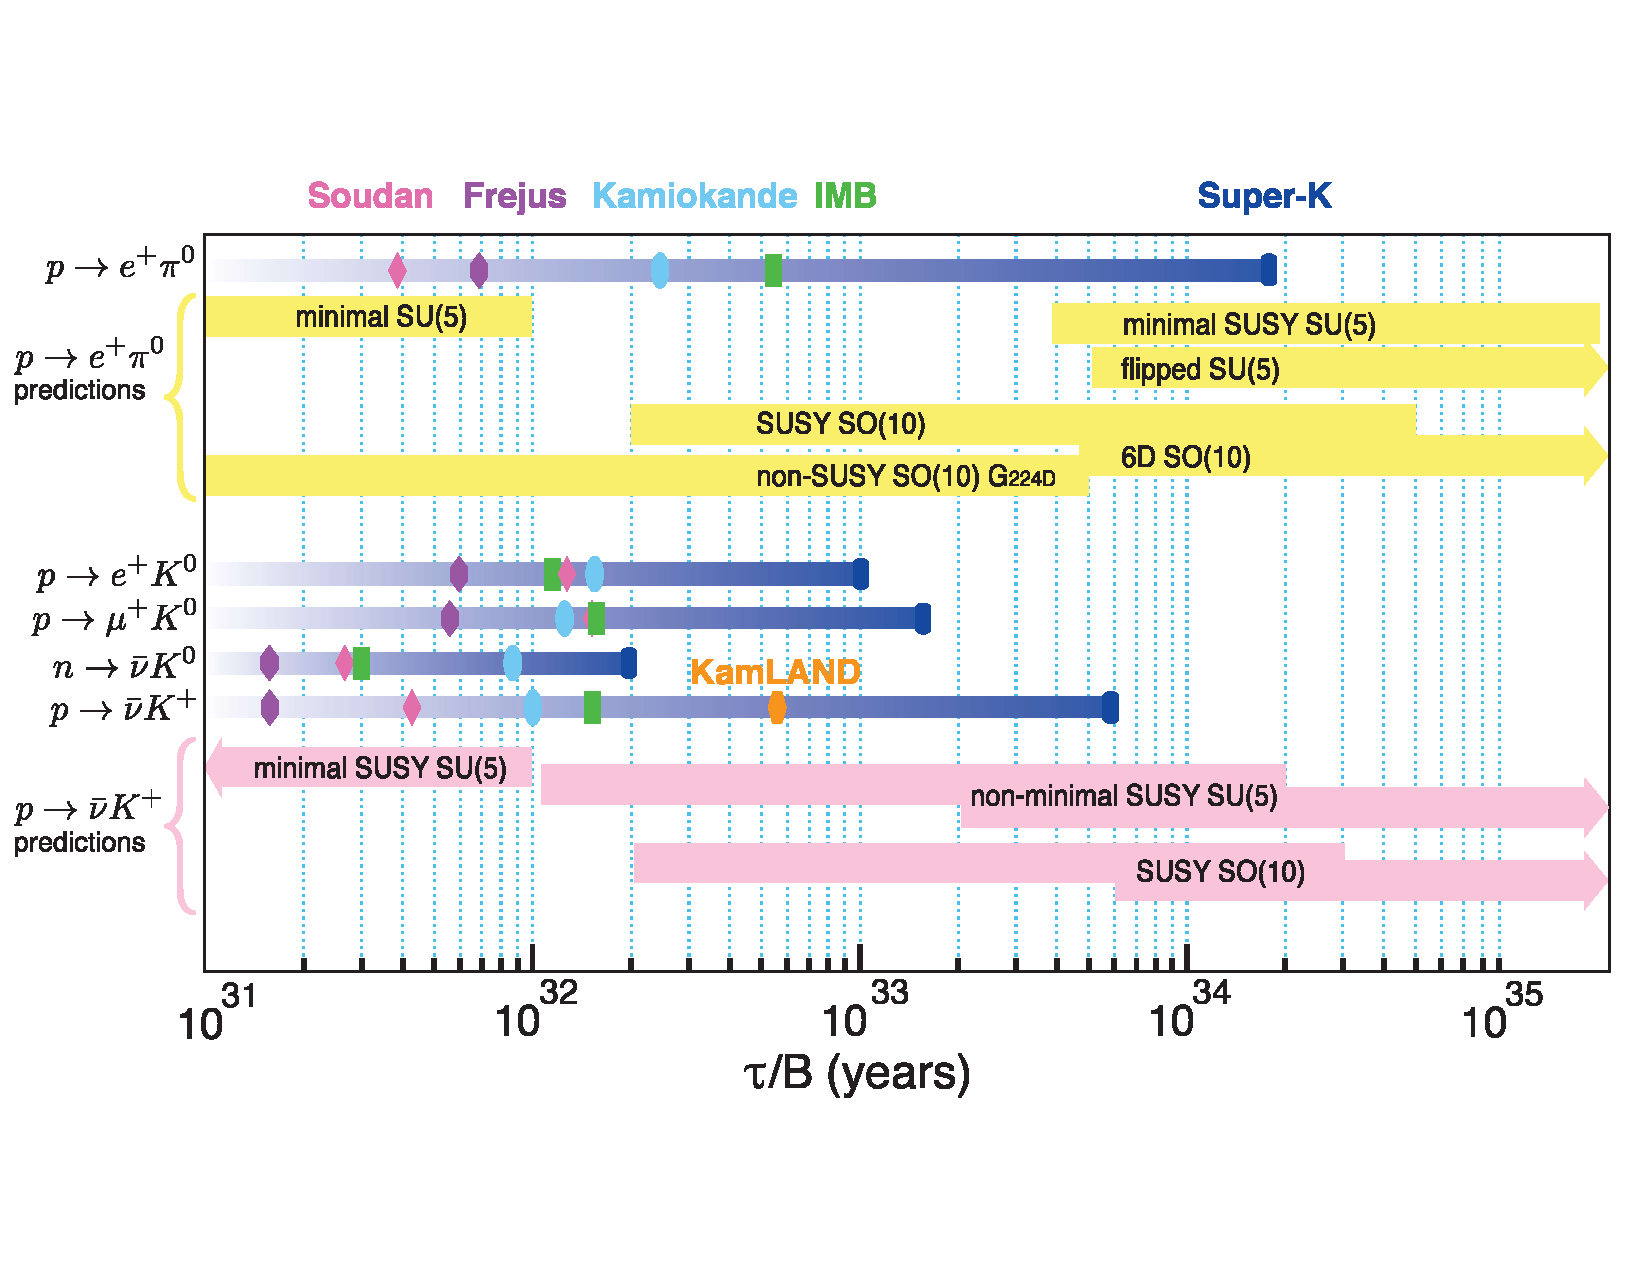
\includegraphics[width=0.9\textwidth]{TheoryExpLimitSummary.pdf}
\end{dunefigure}

\subsection{Experimental Signatures for Nucleon Decay Searches in DUNE}
\label{subsec:nonaccel-ndk-dune}

The DUNE far detector, with the largest active volume of argon, 
will be highly sensitive to several possible nucleon decay modes, 
in many cases complementing the capabilities of large water detectors.
In particular, \lartpc technology offers the opportunity to observe the entire decay chain for nucleon decays into charged kaons; in $p \rightarrow \bar{\nu}K^{+}$, the kaon is typically below \cherenkov threshold in a water \cherenkov detector, but can be identified by its distinctive $dE/dx$ signature as well as by its decay in a \lartpc.
Therefore, this mode can be tagged in a \lartpc if a single kaon within a proper energy/momentum range can be reconstructed with its point of origin lying within the fiducial volume followed by a known decay mode of the kaon.
Background events initiated by cosmic-ray muons can be controlled  by requiring no activity close to the edges of the \dword{tpc}s and by stringent single kaon identification within the energy range of interest~\cite{bib:docdb3384,bib:docdb1752}.  Atmospheric neutrinos make up the dominant background.

Because of the already stringent limits set by \superk on $p \rightarrow e^{+}\pi^0$ and the unique ability to track and identify kaons in a \lartpc, the initial nucleon decay studies in DUNE have focused on nucleon decay modes featuring kaons.  Studies of $p \rightarrow e^{+}\pi^0$ have begun (see Section~\ref{subsec:nonaccel-ndk-other}) but are less sophisticated than the kaon studies.  The remainder of this section describes the background assumptions, signal simulation, particle tracking and identification, and event classification with a focus on nucleon decay via kaons.

\subsubsection{Background Simulation}
\label{sec:ndkbkgd}

The main background for nucleon decay searches is in the interactions of  atmospheric neutrinos. In this analysis, the Bartol flux~\cite{Barr:2004br} is used.
%\cite{Bartolref} at Soudan location is used, the Bartol flux is a MC calculation of the atmospheric neutrino fluxes, the calculations starts with simulations of the interactions of the primary cosmic rays with the atmosphere. The earth is assumed to be a sphere and primaries are generated with random positions and angles. The effect of the geomagnetic field on the interacting cosmic rays is included by applying the cutoff using the back-tracing technique \cite{Bartolref} . 
%Fig \ref{fig:atmo_flux} shows the atmospheric flux prediction for different neutrino species.
Neutrino interactions in argon are simulated with the GENIE Neutrino Monte Carlo Generator~\cite{Andreopoulos:2009rq}. To estimate the event rate, we integrate the product of the neutrino flux and interaction cross-section.
Table \ref{tab:rate} shows the event rate for different neutrino species for an exposure of 10~kton$\cdot$years.

\begin{dunetable}
[Expected rate of neutrino interactions in $^{40}$Ar for 10~kton-year exposure.]
{cccc}
{tab:rate}
{Expected rate of neutrino interactions in $^{40}$Ar for a 10~kton-year exposure.}
  ~10~kton-years~   &~CC~&~NC~&~Total \\
$\nu_{\mu}$ & 1038 & 398 &1436 \\
$\bar{\nu}_{\mu}$ &280 & 169 & 449 \\
$\nu_{e}$ & 597 &  206 &83 \\
$\bar{\nu}_{e}$ & 126 & 72 & 198 \\
Total & 2014 & 845 & 2886 \\
\end{dunetable}

Thus, to suppress atmospheric neutrino background to the level of 1 event per Mton-year, which would yield 0.4 events after ten years of operation with a 40-kton fiducial volume, the rejection factor needed is $3\times 10^{-6}$.

\subsubsection{Nucleon Decay Simulation}
\label{sec:ndksim}

The simulation of nucleon decay events is performed using GENIE v.2.12.10. 
A total of 68 single-nucleon exclusive decay channels listed in the 2016 update of the \dword{pdg}~\cite{Patrignani:2016xqp} is available in GENIE (see Table~\ref{tab:genie-ndk} 
in Appendix~\ref{sec:tools-app-generator}). The list includes two-, three-, and five-body decays. 
%The numbering in the decay modes follows the PDG convention. 
%The primary decay is simulated using a phase-space-decay generator. 
%For bound nucleons, the nuclear environment is simulated as in neutrino scattering. 
%The nucleon is assigned a Fermi momentum and removal energy and it is off the mass shell.  
%The relativistic Fermi gas (RFG) nuclear model is used with a Bodek-Ritchie  tail to incorporate short range nucleon-nucleon correlations \cite{Bodek:1981wr}. 
%For $^{40}$Ar the Fermi momentum has a default value of 242.0 MeV/c with binding energy = 27.0 MeV. 
If a bound nucleon decays, the remaining nucleus can be in an excited state and will typically de-excite by emitting nuclear fission fragments, nucleons, and photons. At present, de-excitation photon emission is simulated only for oxygen~\cite{Andreopoulos:2015wxa}.  However, the \argoneut collaboration~\cite{Acciarri:2018myr} has reported measurements of argon de-excitation gamma in \lartpc detectors,
where energy depositions and positions of these depositions have been compared to those from simulations of neutrino-argon interactions using the FLUKA Monte Carlo generator.

\subsubsection{Kaon Final State Interactions}
\label{sec:final-state-interactions}

The propagation of the decay products in the nucleus is simulated using an intra-nuclear cascade \dword{mc}. 
%The probability $\lambda$ that a particle will undergo an interaction is governed by the free cross section $\sigma$ and the density of nucleons $\rho$,
%\begin{equation}
%\lambda(E,r)= \frac{1}{\sigma \rho(r)}.
%\end{equation}
%The type of interaction is then chosen according to the cross sections for various reactions for free nucleons, sometimes modified for nuclear medium effects, relative to the total cross section. 
Charged kaons can undergo various scattering processes in the nucleus: elastic scattering, charge exchange, absorption (only $K^{-}$; $K^{+}$ absorption is forbidden), and $K^{+}$ production via strong processes such as $\pi^{+}n \rightarrow K^{+} \Lambda$.  In this analysis, the $hA2015$ model in GENIE is used as the default model for these \dword{fsi}.  $hA2015$ is an empirical, data-driven method that does not model the cascade of hadronic interactions step by step, but instead uses one effective interaction where hadron+nucleus data is used to determine the final state.
For kaons, $K^{+}+C$ data~\cite{Bugg:1968zz,Friedman:1997eq}
is used when available. $hA2015$ only considers kaon-nucleon elastic scattering inside the nucleus.  Charge exchange is not included, nor is $K^+$ production in pion reactions, and therefore a $K^+$ is never added or removed from the final state in this model. Other \dword{fsi} models include the full cascade, but there is not enough data to favor one model over the other.  For example, a measurement of kaon production in neutrino interactions shows only a weak preference for including \dword{fsi} as opposed to a model with no \dword{fsi}~\cite{Marshall:2016rrn}.

\dword{fsi} can significantly modify the observable distributions in the detector.  For example, Figure \ref{fig:K-wFSI-hA2015} shows the kinetic energy of a kaon from $p\rightarrow \bar{\nu}K^{+}$ before and after \dword{fsi}. Because of \dword{fsi} the kaon spectrum becomes softer on average. Of the kaons, 31.5$\%$  undergo elastic scattering resulting in events with very low kinetic energy;  $25\%$ of kaons have a kinetic energy of $\le$50 MeV. When the kaon undergoes elastic scattering, a nucleon can be knocked out of the nucleus. Of decays via this channel, $26.7\%$  have one neutron coming from \dword{fsi}, $15.3\%$ have at least one proton, and $10.3\%$ have two protons coming from \dword{fsi}. These secondary nucleons are detrimental to reconstructing and selecting  $K^{+}$.

\begin{dunefigure}[Kaon kinetic energy before and after FSI]{fig:K-wFSI-hA2015}{Kinetic energy of kaons in simulated proton decay events, $p\rightarrow K^{+} \bar{\nu}$.  The kinetic energy distribution is shown before and after final state interactions in the argon nucleus.}
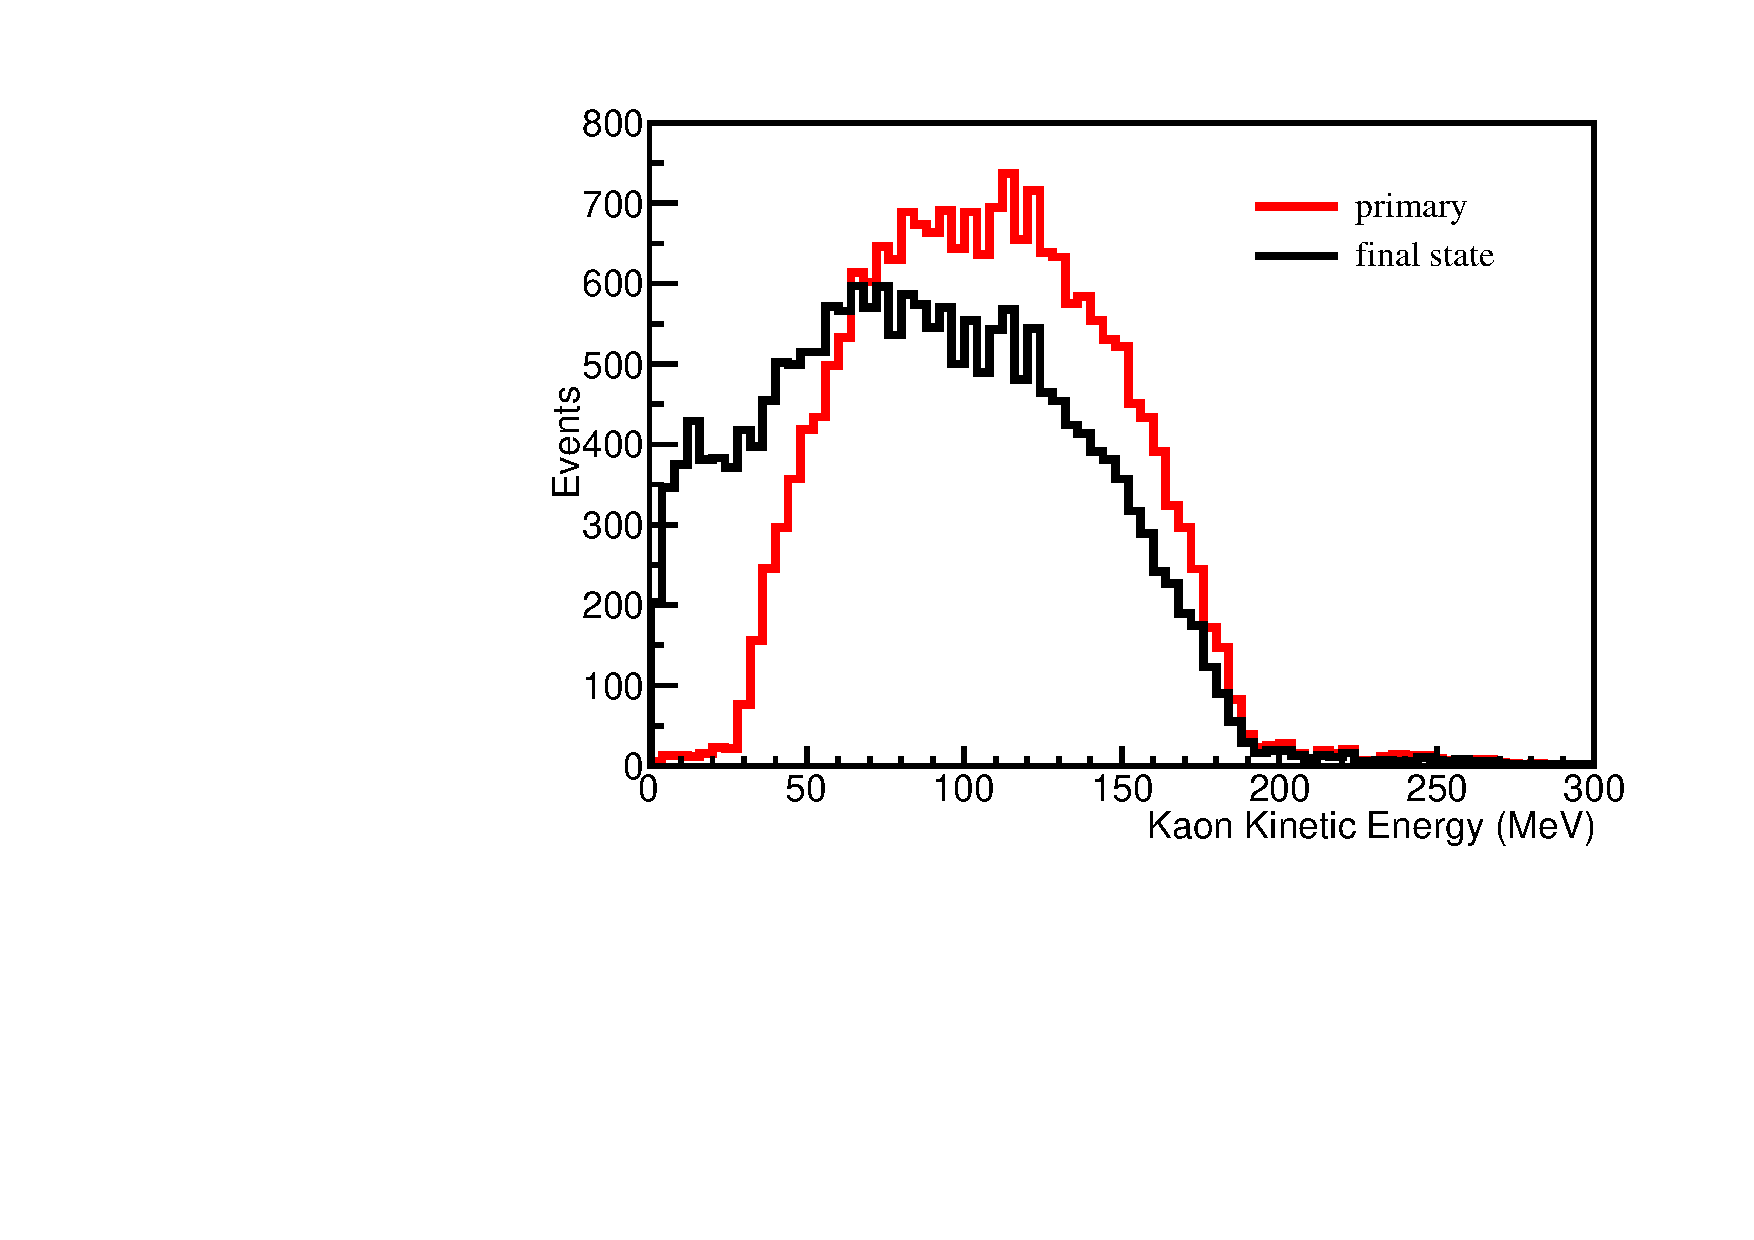
\includegraphics[width=0.8\textwidth]{K-wFSI-hA2015.pdf}
\end{dunefigure}

The kaon \dword{fsi} in \superk's simulation of $p\rightarrow K^{+} \bar{\nu}$ in oxygen seem to have a smaller effect on the outgoing kaon momentum distribution~\cite{Abe:2014mwa} than is seen here with the GENIE simulation on argon.  Some differences are expected due to the different nuclei, but differences in the \dword{fsi} models are under investigation.

\subsubsection{Tracking and Particle Identification}
\label{sec:event-reconstruction}

The DUNE reconstruction algorithms are described in Chapter~\ref{ch:tools}.  This analysis uses \threed track and vertex reconstruction provided by \dword{pma}.
%\fixme{This is not in the glossary.}

Track reconstruction efficiency for a charged particle $x^{\pm}$ is defined as 

\begin{equation}
\epsilon_{x^{\pm}} = \frac{\mbox{$x^{\pm}$ particles with a reconstructed track}}{\mbox{events with $x^{\pm}$ particle }}.
\end{equation}
The denominator includes events in which an $x^{\pm}$ particle was created and has deposited energy within any of the \dwords{tpc}.  The numerator includes events in which an $x^{\pm}$ particle was created and has deposited energy within any of the \dwords{tpc}, and a reconstructed track can be associated to the $x^{\pm}$ particle based on the number of hits generated by that particle along the track. This efficiency can be calculated as a function of true kinetic energy and true track length.

\begin{dunefigure}[Tracking efficiency of kaons in $p\rightarrow K^{+} \bar{\nu}$]{fig:k-trk-eff}{Tracking efficiency for kaons in simulated proton decay events, $p\rightarrow K^{+} \bar{\nu}$, as a function of kaon kinetic energy (left) and true path length (right).}
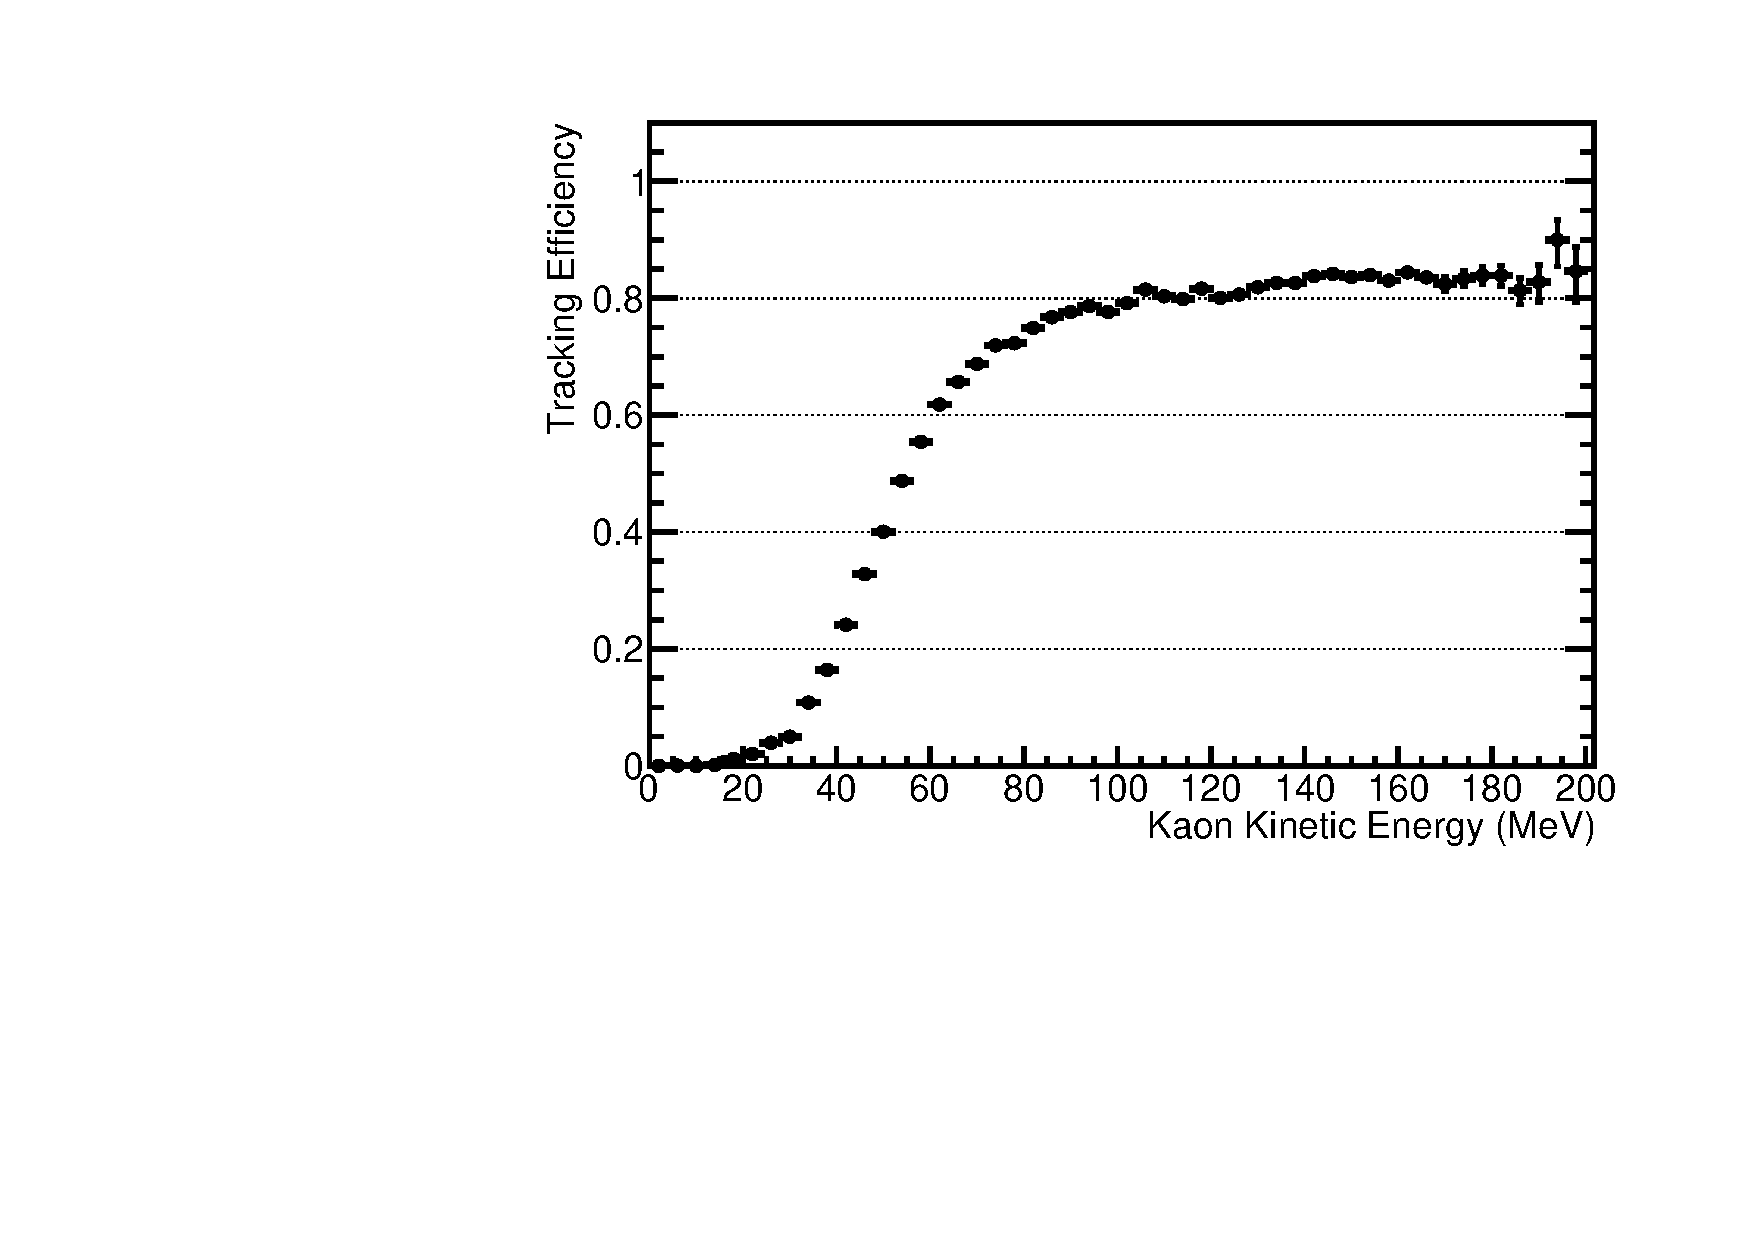
\includegraphics[width=0.4\textwidth]{k-trk-eff-KE.pdf}
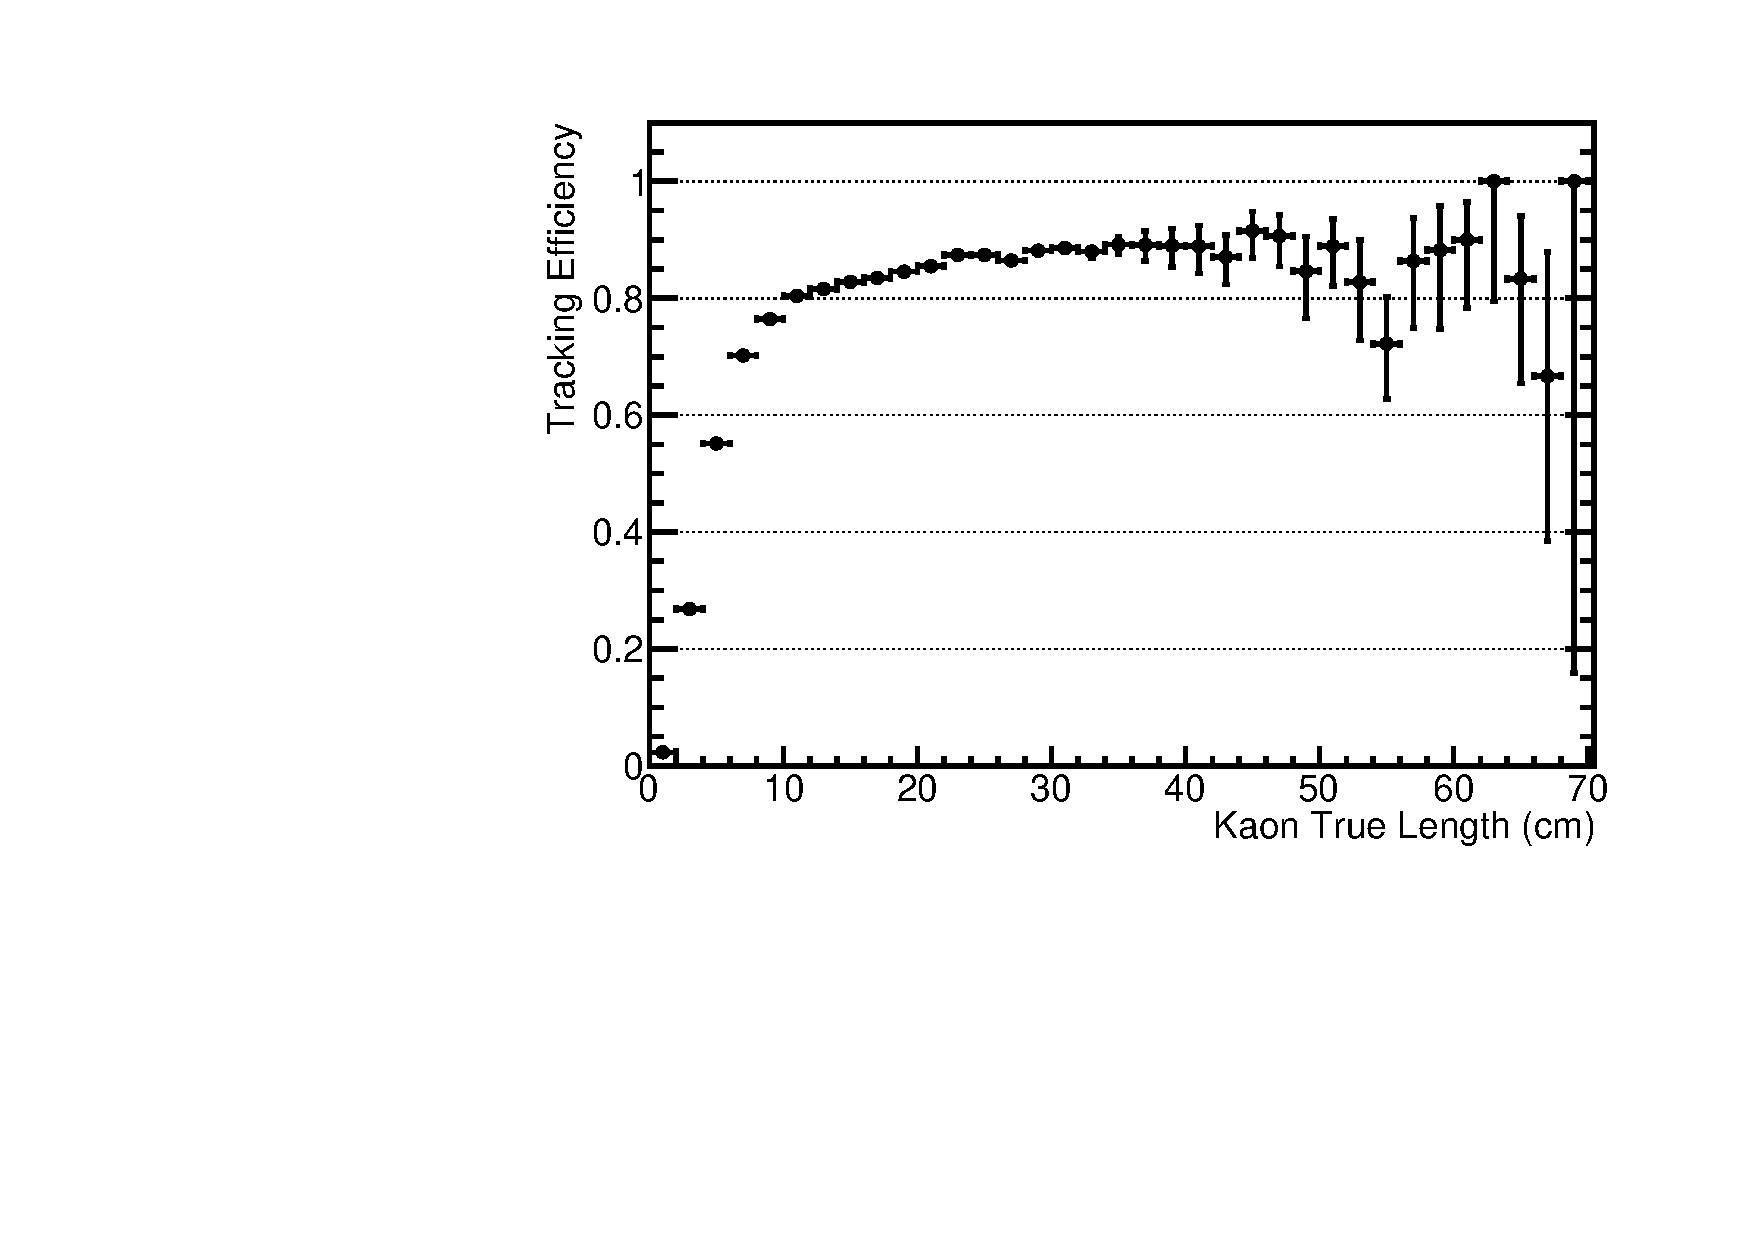
\includegraphics[width=0.4\textwidth]{k-trk-eff-length.pdf}
\end{dunefigure}

Figure \ref{fig:k-trk-eff} shows the tracking efficiency for $K^{+}$  from proton decay via $p\rightarrow \bar{\nu}K^{+}$ as a function of true kinetic energy and true path length. The overall tracking efficiency for kaons is 58.0$\%$, so 58.0\% of the simulated kaons are associated with a reconstructed track in the detector.  From Figure~\ref{fig:k-trk-eff}, the tracking threshold is approximately $\sim$40~MeV of kinetic energy, which translates to $\sim$4.0~cm in true path length.  The biggest loss in tracking efficiency is due to kaons with $<40$~MeV of kinetic energy due to scattering inside the nucleus as described in Section~\ref{sec:final-state-interactions}.  The efficiency levels off to approximately $80\%$ above 80~MeV of kinetic energy; this inefficiency even at high kinetic energy is due mostly to kaons that decay in flight.
Both kaon scattering in the \dword{lar} and charge exchange are included in the simulation but are relatively small effects (4.6\% of kaons scatter in the \dword{lar} and 1.2$\%$ of kaons experience charge exchange).   

%%%%%%%%%%%
%\todo{remove completeness and purity discussion to save space?}
%Another useful metric in evaluating tracking performance is the completeness and purity of the track. Completeness is defined as

 %\begin{equation}
%Completeness = \sum_{i}^{\mbox{track hits}}\frac{\mbox{(hit energy on track %from a charged particle)}_{i}}{\mbox{total hit energy from a charged %particle}},
%\end{equation}
%where completeness equal to one means all hits associated with a charged particle were reconstructed as a single track. 
%Figure \ref{fig:k_complet_purity} (left) shows track completeness for $K^{+}$ from proton decay events via $p\rightarrow \bar{\nu}K^{+}$. The peak at 0.6 is due to the three-plane design of the \dword{tpc}.  If a particle travels parallel to a wire plane, very likely the reconstruction algorithm cannot match the \twod clusters of hits in all three views.  This results in a track with a completeness of 2/3 (0.667), with 1/3 of the hits not associated to the track.  This feature affects particle identification because it causes mis-reconstruction of the decay point, where the $dE/dx$ information is most useful.

%Track purity is the estimated level of hit contamination from another %particle, defined as

%\begin{equation}
%Purity = \sum_{i}^{\mbox{track hits}}\frac{\mbox{(hit energy on track from a charged particle)}_{i}}{\mbox{total hit energy on the track}},
%\end{equation}

%Figure \ref{fig:k_complet_purity} (right) shows the track purity for $K^{+}$ from proton decay events via $p\rightarrow \bar{\nu}K^{+}$. The average purity for a kaon track is approximately 0.94. 
%Of kaon tracks, 16$\%$ have lower than average purity; in most cases, this is due to a proton and kaon overlapping in a single track. This also affects particle identification; the information on $dE/dx$ is misleading because of the overlap of a different particle. 

%\begin{dunefigure}[Completeness and purity of kaon tracks in $p\rightarrow K^{+} \bar{\nu}$]{fig:k_complet_purity}{Completeness (left) and purity (right) for kaon tracks in simulated proton decay events, $p\rightarrow K^{+} \bar{\nu}$.}
%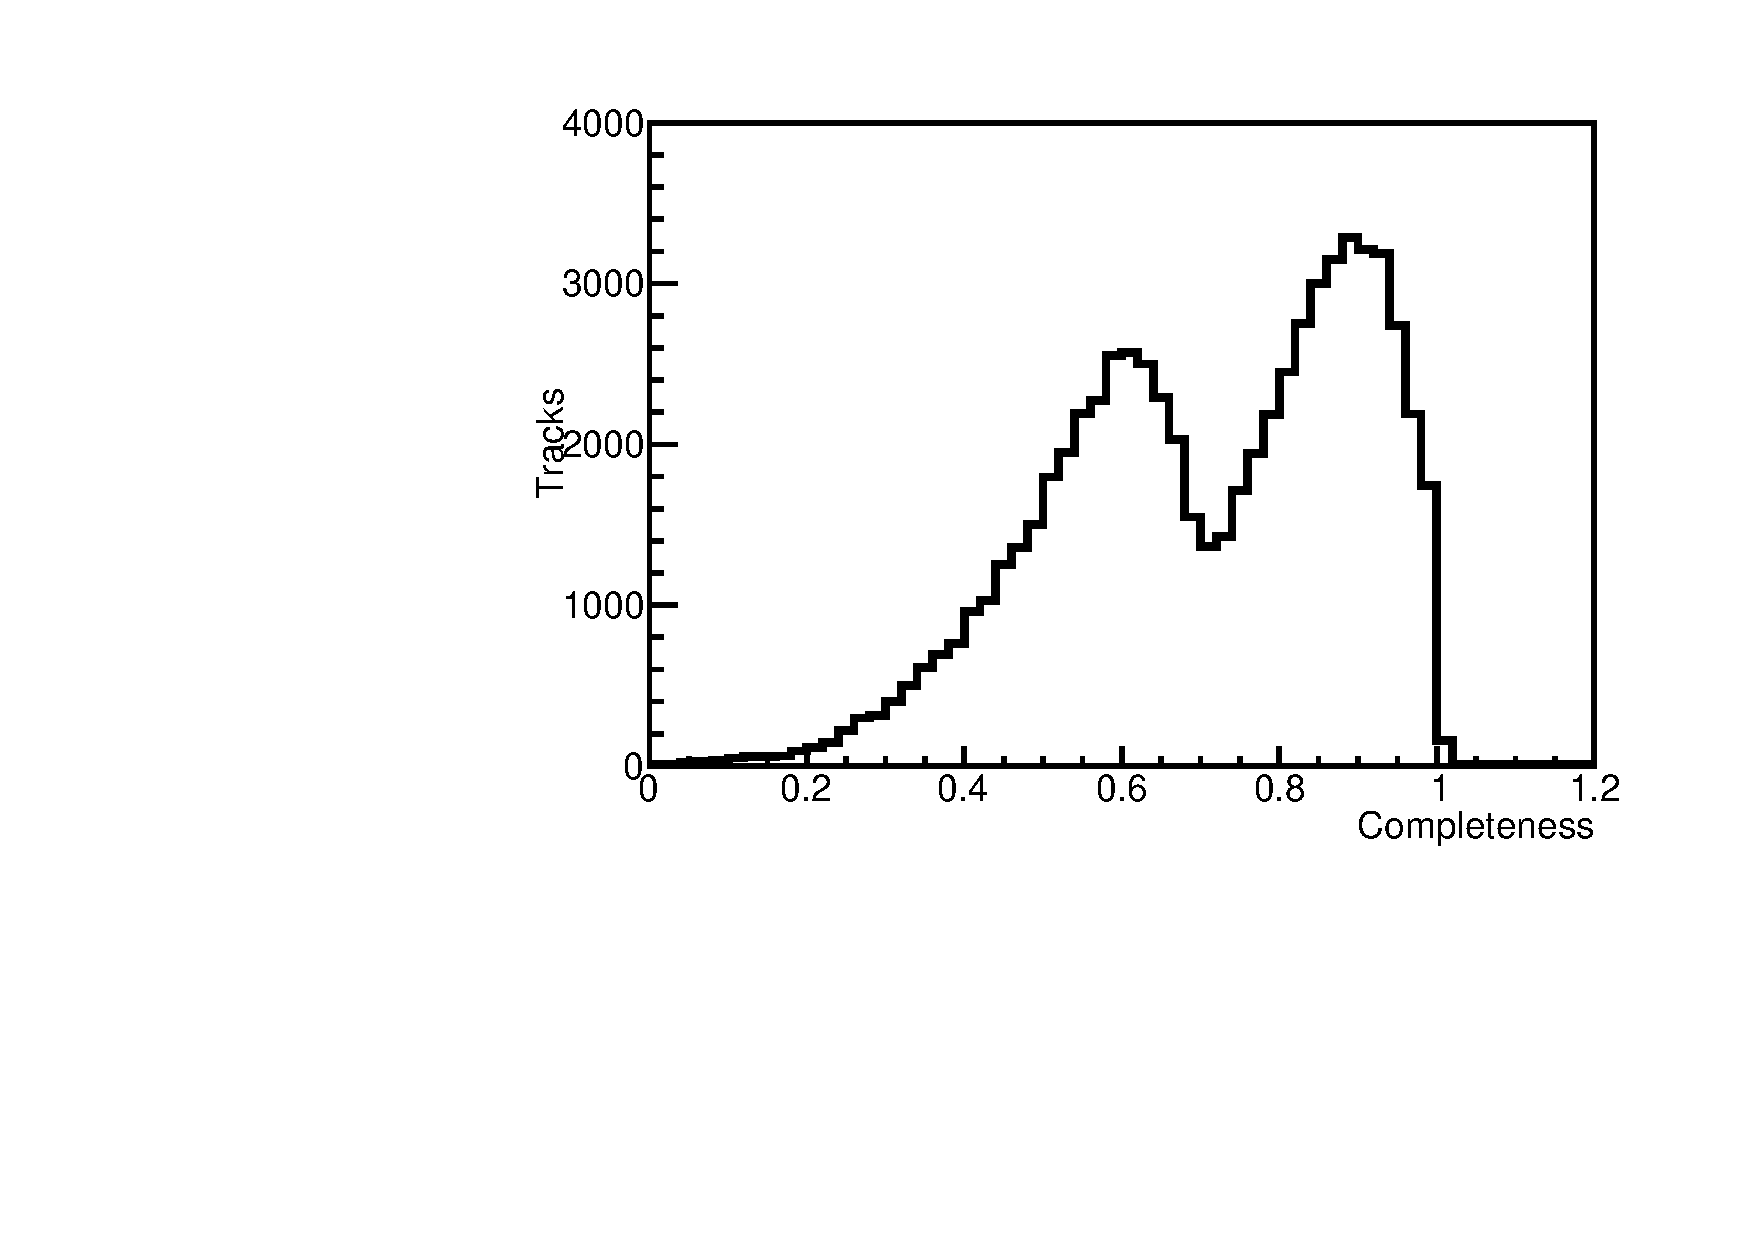
\includegraphics[width=0.49\textwidth]{k_complet.pdf}
%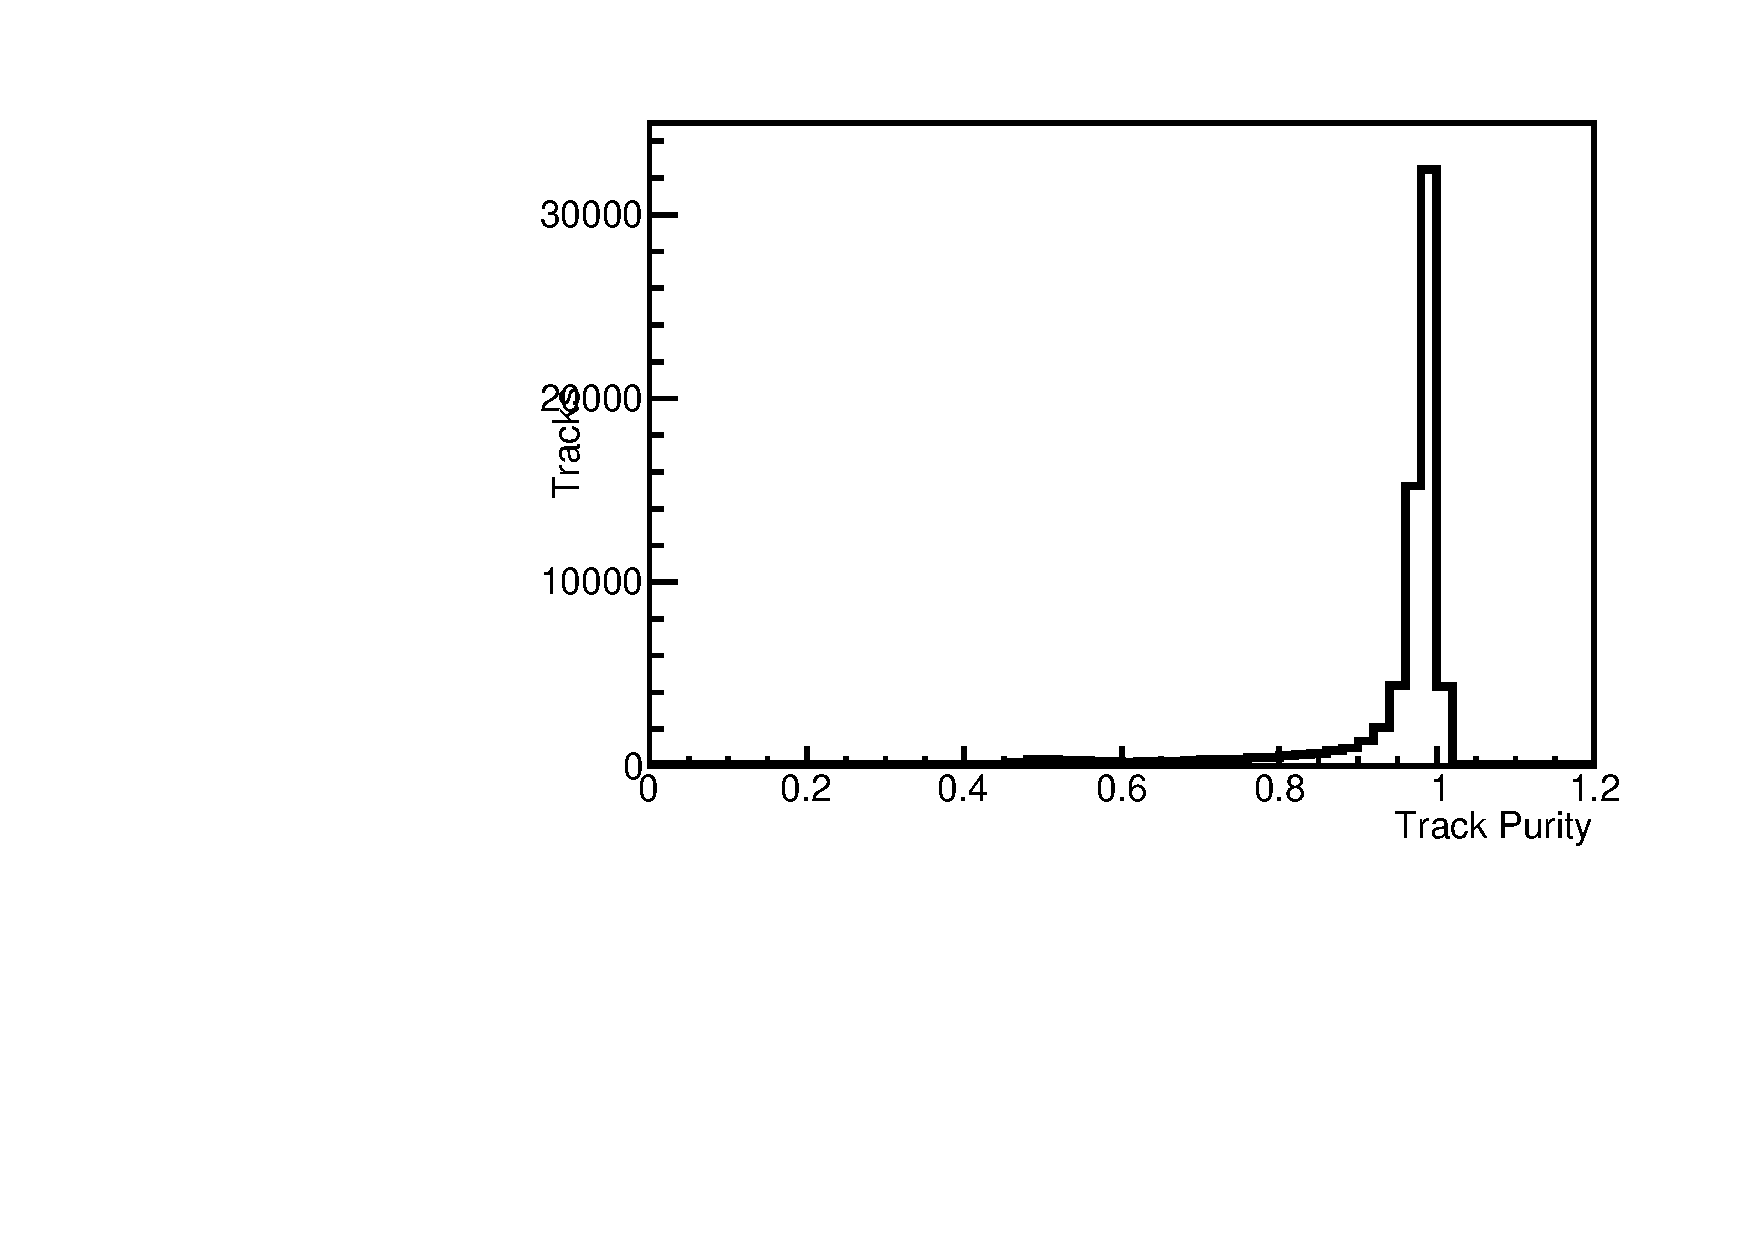
\includegraphics[width=0.49\textwidth]{k_purity.pdf}
%\end{dunefigure}
%%%%%%%%%%%%%%%

Charged particles lose energy through ionization and scintillation when traversing the \dword{lar}. This energy loss provides valuable information on particle energy and species. To identify a given particle, the hits associated with a reconstructed track are used.
The total energy deposition from the track is obtained by summing the $dE/dx$ for all reconstructed hits. 
If the charged particle stops in the \lartpc active volume, a combination of $dE/dx$ and the reconstructed residual range ($R$, the path length to the end point of the track) is used to define a parameter for \dword{pid}.  The parameter, $PIDA$, %\fixme{This abbreviation (PIDA) is not in the glossary. There is a PID, which is apparently what you mean here.} 
%PIDA is a variable name, not an abbreviation.  PIDA is a variable that is used to perform particle identification (PID).  I put PIDA in math mode, like dE/dx, to make that clear.
is defined as  

\begin{equation}
PIDA = \left\langle \left(\frac{dE}{dx}\right)_{i}R^{0.42}_{i}\right\rangle,\label{eqn:PIDA}
\end{equation}
where the median is taken over all track points $i$ for which the residual range $R_i$ is less than 30~cm.
%This procedure can be done for each plane. 

\begin{dunefigure}[Particle identification using $PIDA$ for $p\rightarrow K^{+} \bar{\nu}$]{fig:PIDA}{Particle identification using $PIDA$ for particles in simulated proton decay events, $p\rightarrow K^{+} \bar{\nu}$.}
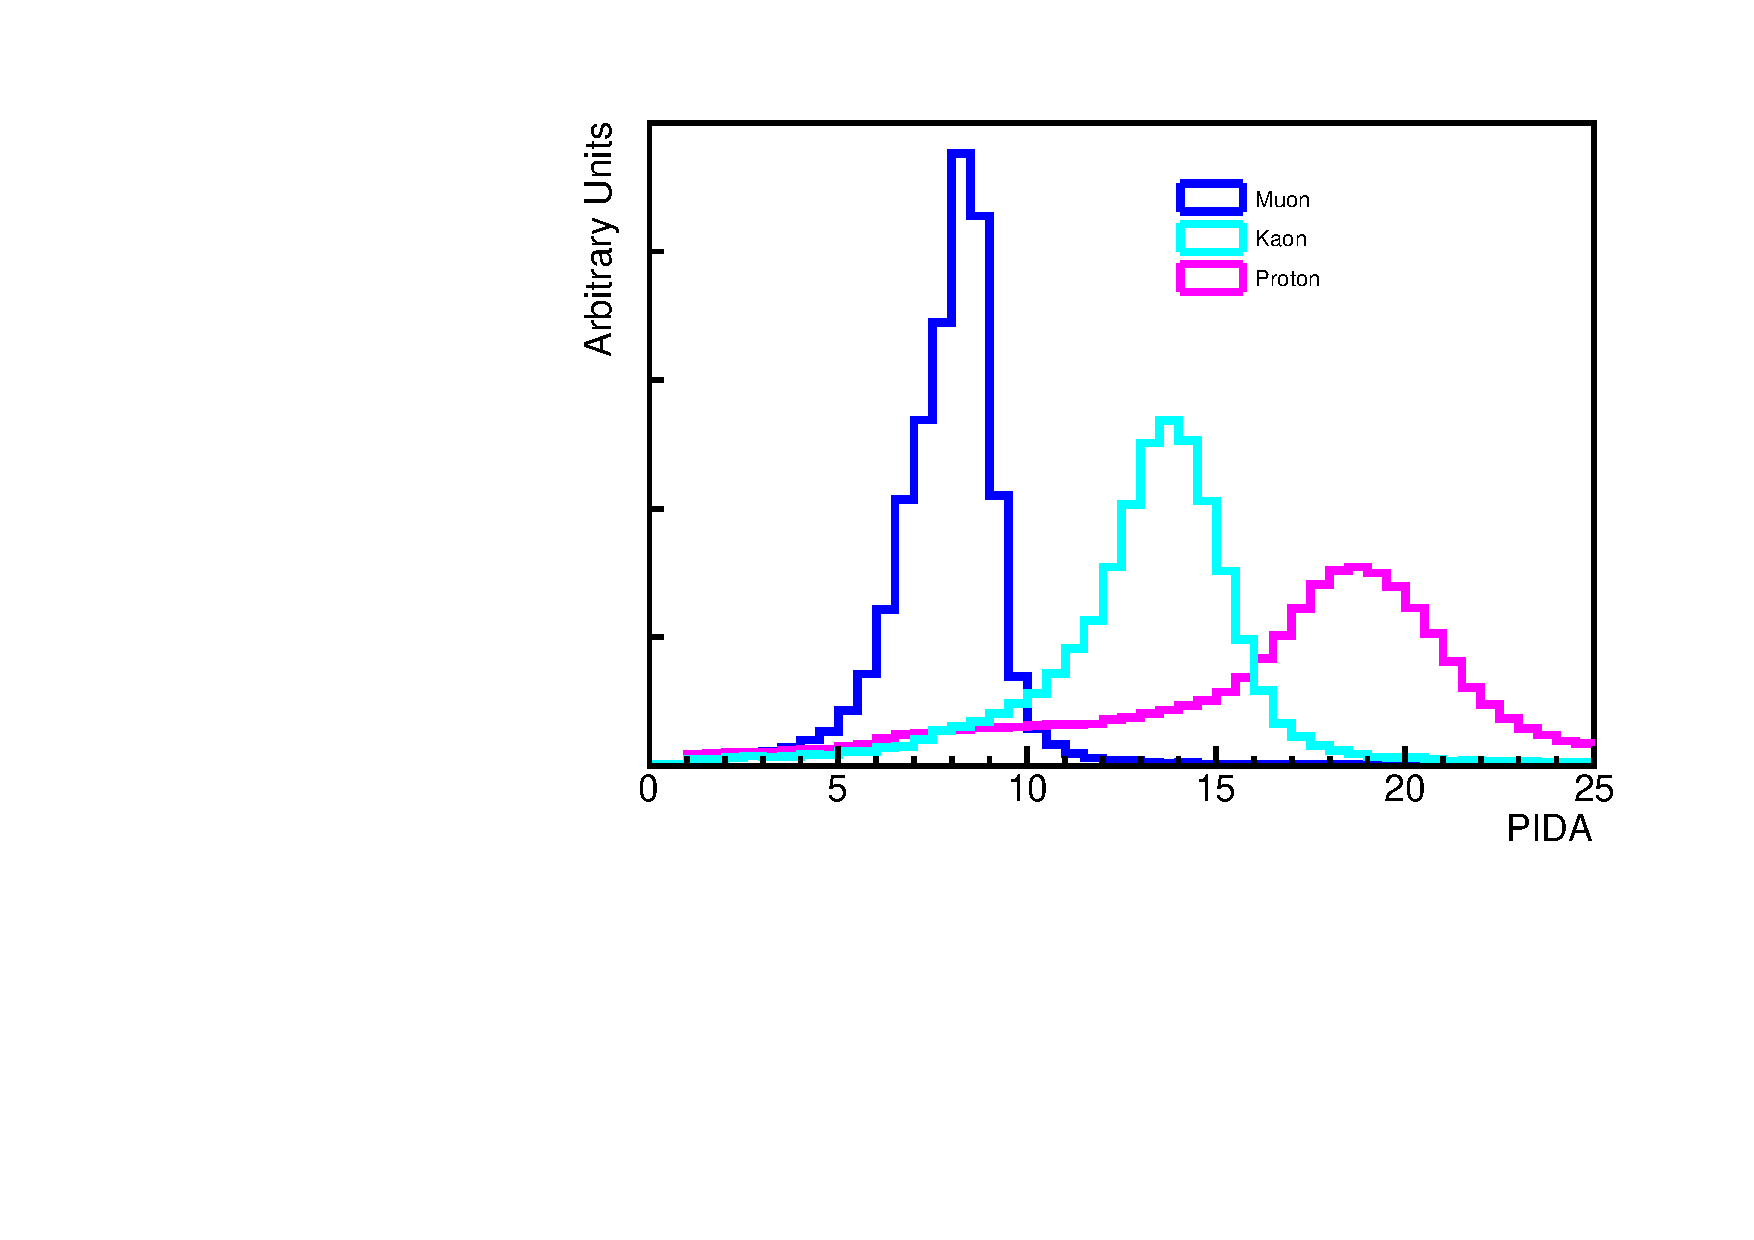
\includegraphics[width=0.8\textwidth]{PIDA.pdf}
\end{dunefigure}

Figure \ref{fig:PIDA} shows the $PIDA$ performance for kaons (from proton decay), muons (from kaon decay), and protons produced by atmospheric neutrino interactions. The tail with lower values in each distribution is due to cases where the decay/stopping point was missed by the track reconstruction. The tail with higher values is caused when a second particle overlaps at the decay/stopping point causing higher values of $dE/dx$ and resulting in higher values of $PIDA$. In addition, ionization fluctuations smear out these distributions.

A complication for \dword{pid} via $dE/dx$ results when ambiguity occurs in reconstructing track direction, which is even more problematic because additional energy deposition may occur at the originating point in events where \dword{fsi} is significant.  The dominant background to $p\rightarrow \bar{\nu} K^{+}$ in DUNE is atmospheric neutrino \dword{cc} \dword{qe}
%\fixme{This abbreviation is not in the glossary, although CC is used for charged current. You could use CC quasi-elastic to avoid having yet another abbreviation.} 
%CC and QE are defined separately in the glossary
scattering, $\nu_{\mu} n \rightarrow \mu^{-} p$.  When the muon happens to have very close
to the 237~MeV/c momentum expected from a $K^{+}$ decay at rest and does not capture, it is indistinguishable from the muon resulting from $p\rightarrow \bar{\nu} K^{+}$ followed by $K^{+} \rightarrow \mu^{+}\nu_{\mu}$. When
the proton is also mis-reconstructed as a kaon, this background mimics the signal process.  

The most important difference between signal and this background source is the direction of the hadron track. For an atmospheric neutrino, the proton and muon originate from the same neutrino interaction point, and the characteristic Bragg rise occurs at the end of the proton track farthest from the muon-proton vertex. In signal, the kaon-muon vertex is where the $K^{+}$ stops and decays at rest, so its ionization energy deposit is highest near the kaon-muon vertex.  To take advantage of this difference, a log-likelihood ratio discriminator is used to distinguish signal from background.  Templates are formed by taking the reconstructed calibrated energy deposit as a function of the number of wires from both the start and end of the $K^{+}$ candidate hadron track. 
%The best view is used, which is typically the collection plane. 
Two log-likelihood ratios are computed separately for each track. The first begins at the hadron-muon shared vertex and moves along the hadron track (the ``backward'' direction). The second begins at the other end of the track, farthest from the hadron-muon shared vertex, moves along the hadron track the other way (the ``forward'' direction). For signal events, this effectively looks for the absence of a Bragg rise at the $K^{+}$ start, and the presence of one at the end, and {\it vice versa}
%\fixme{Vice versa should be italicized.} 
for background.  At each point, the probability density for signal and background, $P^{sig}$ and $P^{bkg}$, are determined from the templates. Forward and backward log-likelihood ratios are computed as

\begin{align}
 \mathcal{L}_{fwd(bkwd)} = \sum_{i} \log\frac{P^{sig}_i}{P^{bkg}_i}, 
\end{align}
where the summation is over the wires of the track, in either the forward or backward direction. The discriminator is the sum of the forward and backward log-likelihood ratios:

\begin{align}
    \mathcal{L} = \mathcal{L}_{fwd} + \mathcal{L}_{bkwd}.\label{eqn:L}
\end{align}
Applying this discriminator to tracks with at least ten wires gives a signal efficiency of roughly 0.4 with a background efficiency of 0.01.

\subsubsection{Event Classification}

Multivariate classification methods based on machine learning techniques have become a fundamental part of most analyses in high-energy physics. 
To develop an event selection to search for nucleon decay, a \dword{bdt}
%\fixme{This abbreviation is not in the glossary.} 
classifier is used. The software package Toolkit for Multivariate Data Analysis with ROOT (TMVA4)~\cite{Hocker:2007ht}
was used with AdaBoost as the boosted algorithm.  In the analyses presented here, the \dword{bdt} is trained on a sample of \dword{mc} events (50k events for signal and background) that is statistically independent from the sample of \dword{mc} events used in the analysis (100k events for signal and 600k events for background.)

As an independent method of identifying nucleon decay events, image classification using a \dword{cnn}
%\fixme{Again, the abbreviation is not in the glossary.} 
can be performed using \twod images of DUNE \dword{mc} events. The image classification provides a single score value as a metric of whether any given event is consistent with a proton decay, and this score can be used as a powerful discriminant for event identification.

\subsection{Sensitivity to $p\to K^+\bar{\nu}$ Decay}
\label{subsec:nonaccel-ndk-nubarkplus}

%\fixme{BDT, CCQE, and CNN will have to be corrected in this section to correspond to the glossary. This includes the figure title for figures 1.5, 1.6, and 1.7.}

\dword{mc} studies of the $p\to K^+ \bar{\nu}$ signal and corresponding atmospheric neutrino backgrounds have been carried out with the DUNE multipurpose full event simulation and reconstruction software.  As indicated in Section~\ref{sec:event-reconstruction},
%\fixme{Name the section using the coding.}
they reveal that one of the main challenges in identifying proton decay candidates is due to backgrounds arising from the mis-reconstruction of protons as positive kaons. This happens when a \dword{cc} neutrino interaction produces a muon and a recoiling proton, and the primary vertex for neutrino interaction is mislabeled as a secondary vertex where the kaon decays.  Complicating the ability to reject pathological events of this type is the presence of \dword{fsi}, which can shift the spectrum of kaons toward low energies, with possible concurrent emission of nucleons, which together weaken the otherwise distinct energy and $dE/dx$ signature of the kaon. 

The branching fraction for leptonic decay of charged kaons, $K\rightarrow \mu \nu_{\mu}$, is approximately 64$\%$. The remaining decay modes are semileptonic or hadronic and include charged and neutral pions. The leptonic decay offers a distinguishable topology with a heavy ionizing particle followed by a minimum ionizing particle. In addition, given the kinematics of a proton decay event, 92$\%$ of kaons decay at rest. Using two-body kinematics, the momentum of the muon is approximately 237 MeV/$c$. The reconstructed momentum of the muon offers a powerful discriminating variable to separate signal from background events.  This analysis includes all modes of kaon decay, but the selection strategy so far has focused on kaon decay to muons.

The proton decay signal and atmospheric neutrino background events are processed using the same reconstruction chain and subject to the same selection criteria. There are two pre-selection cuts to remove obvious background. One cut requires at least two tracks, which aims to select events with a kaon plus a kaon decay product (usually a muon).  The other cut requires that the longest track be less than 100~cm; this removes backgrounds from high energy neutrino interactions.  After these cuts, 50$\%$ of the signal and 17.5$\%$ of the background remain in the sample.  The signal inefficiency at this stage of selection is due mainly to the kaon tracking efficiency.

A \dword{cnn} was developed to classify signal and background events that give 99.9\% background rejection at 6\% signal efficiency.  Better discriminating power is achieved using a \dword{bdt} with 14 input variables, including the \dword{cnn} score as one  variable.  The other variables in the \dword{bdt} include numbers of reconstructed objects (tracks, showers, vertices), variables related to visible energy deposition, \dword{pid} variables ($PIDA$, Equation~\ref{eqn:PIDA}, and $\mathcal{L}$, Equation~\ref{eqn:L}), reconstructed track length, and reconstructed momentum.
%Including the CNN score in the BDT analysis gives a 40\% background reduction.
Figure \ref{fig:BDT_response} shows the distribution of the \dword{bdt} output for signal and background.

\begin{dunefigure}
[Boosted Decision Tree response for $p\rightarrow K^{+} \bar{\nu}$ ]{fig:BDT_response}
{Boosted Decision Tree response for $p\rightarrow K^{+} \bar{\nu}$ for signal (blue) and background (red).}
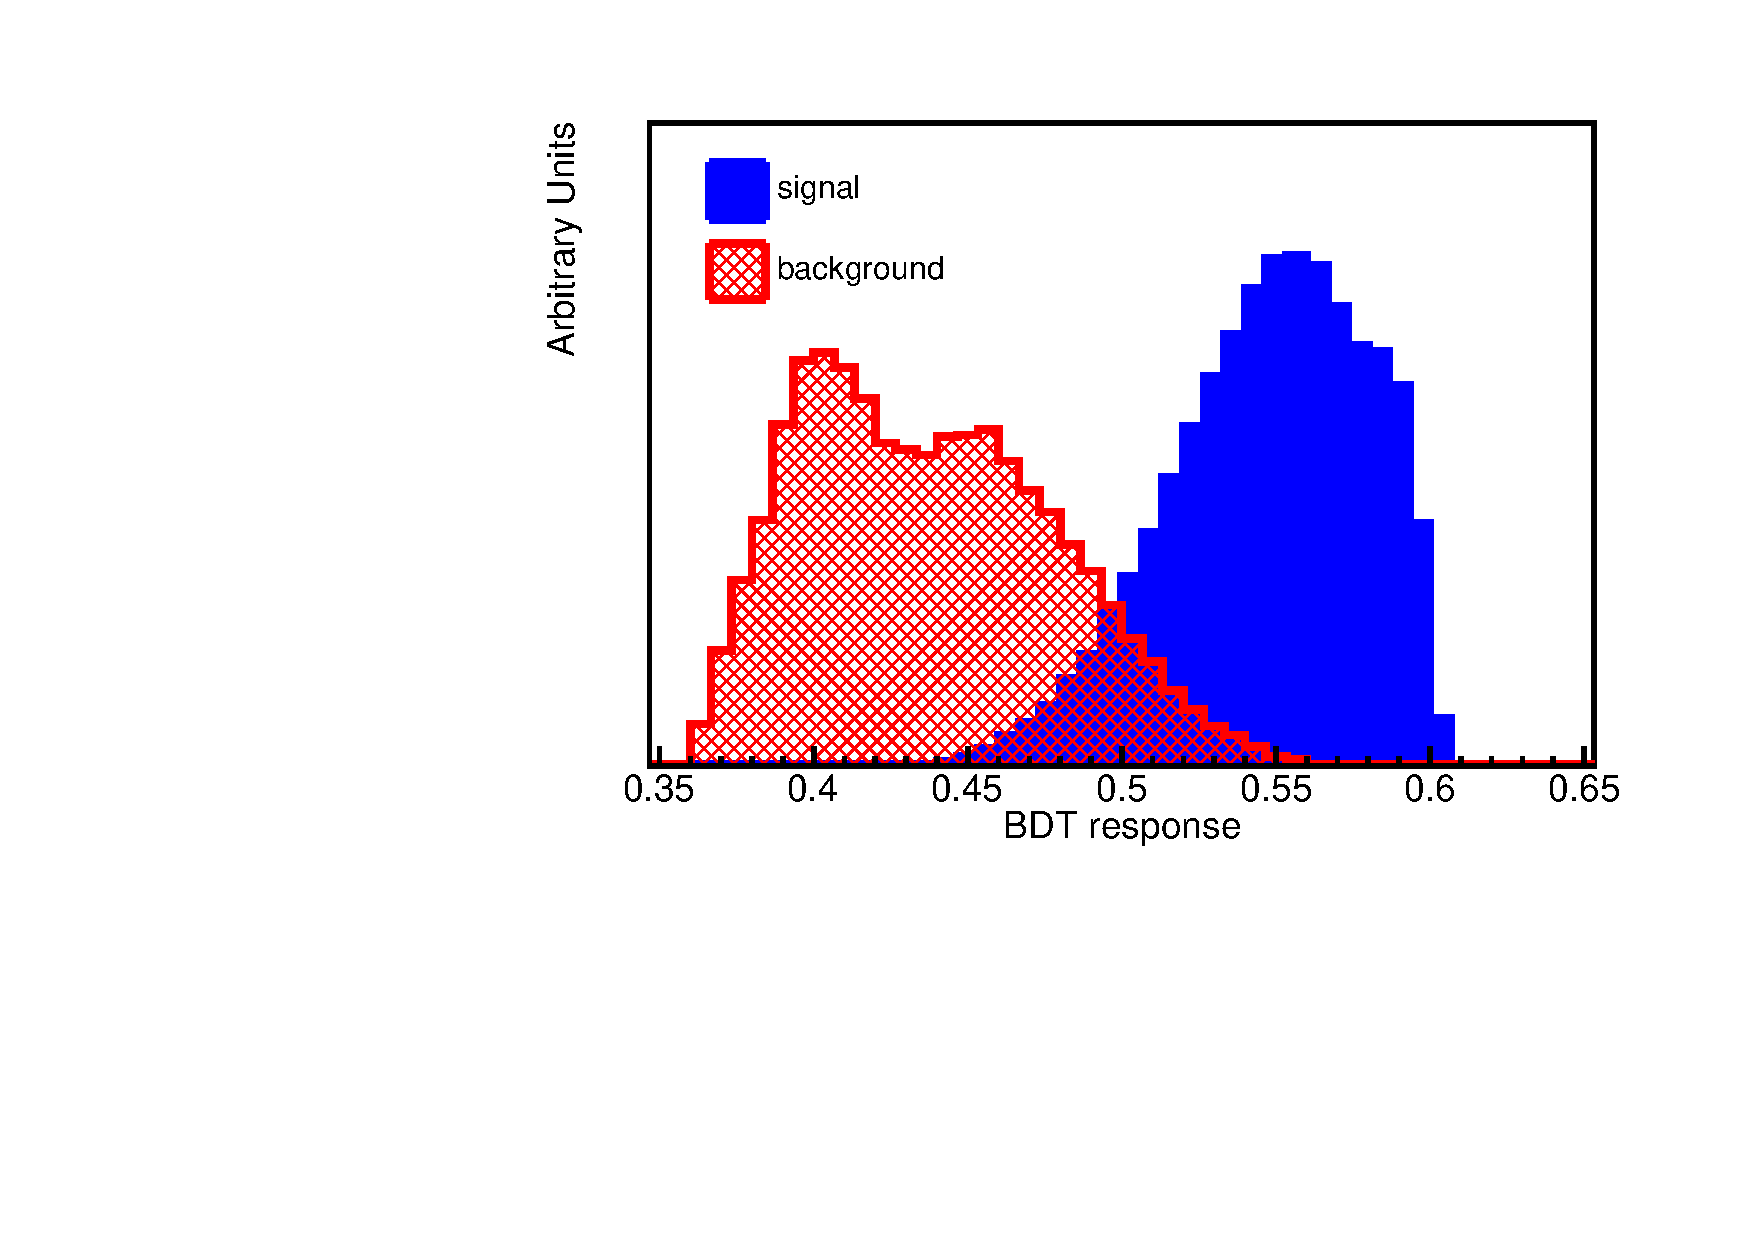
\includegraphics[width=0.8\textwidth]{BDT_response.pdf}
\end{dunefigure} 

%Figure~\ref{fig:BDT_eff} shows the efficiency of the BDT selection for pre-selected signal and background events, where the efficiency is defined as the fraction of true signal or background events remaining in the simulated sample after the cut. The total efficiency can be calculated by multiplying the pre-selection efficiency by the BDT efficiency.  (For example, for a BDT signal efficiency of 30\%, the background BDT efficiency is $\sim 10^{-5}\%$.  The overall efficiency is $15\% = 30\% \times 50\%$ for signal and $\sim10^{-6} \% = 17.5\% \times \sim 10^{-5}\%$ for background, equivalent to $\sim$1 background event per Mton-year.) 
%\todo{clarify bkgd eff/number}

%\begin{dunefigure}
%[BDT efficiency for signal and background]{fig:BDT_eff}
%{BDT selection efficiency for $p\rightarrow K^{+} \bar{\nu}$ signal and background}
%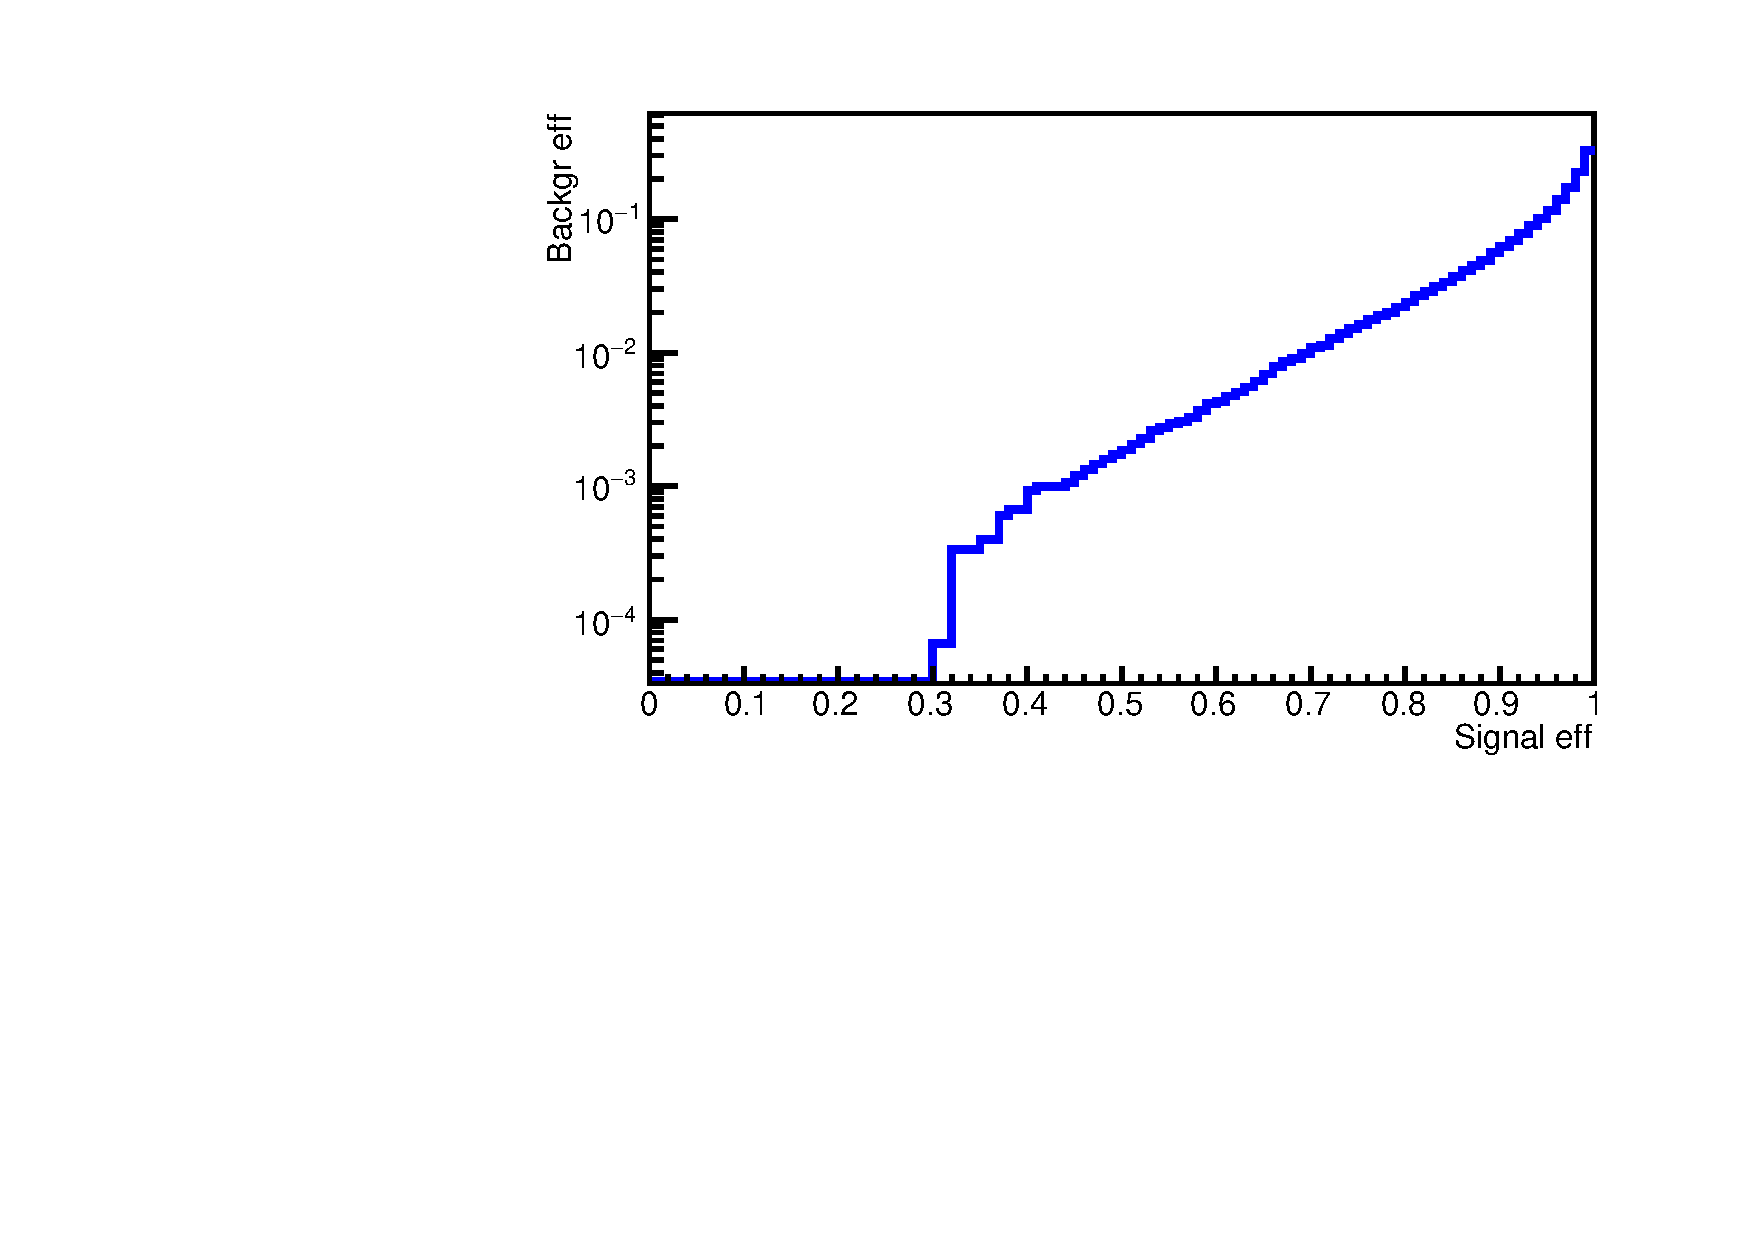
\includegraphics[width=0.8\textwidth]{BDT_eff.pdf}
%\end{dunefigure} 

Figure~\ref{fig:event_signal} shows a signal event with high \dword{bdt} response value (0.605), meaning a well-classified event. The event display shows the reconstructed kaon track in green, the reconstructed muon track from the kaon decay in maroon, and the reconstructed shower from the Michel electron coming from the muon decay in red. Figure~\ref{fig:event_bkgd} shows event displays for background events.  The left figure (\dword{bdt} response value of 0.394) shows the interaction of an atmospheric electron neutrino, $\nu_{e}+n\rightarrow e^{-}+p+\pi^{0}$. The right figure (\dword{bdt} response value 0.587) shows a CCQE interaction of an atmospheric muon neutrino, $\nu_{\mu}+n \rightarrow \mu^{-}+p$. The interaction on the right might be a challenge if the proton track is misidentified as kaon. A tight cut on \dword{bdt} response can remove most of these events, but this significantly reduces signal efficiency.


\begin{dunefigure}
[$p\rightarrow K^{+} \bar{\nu}$ signal event display]{fig:event_signal}
{Event display for a well-classified $p\rightarrow K^{+} \bar{\nu}$ signal event.  The vertical axis is time ticks (each time tick corresponds to 500 ns), and the horizontal axis is wire number. The bottom view is induction plane 1, middle is induction plane 2 and top is the collection plane. The color represents the charge deposited in each hit.}
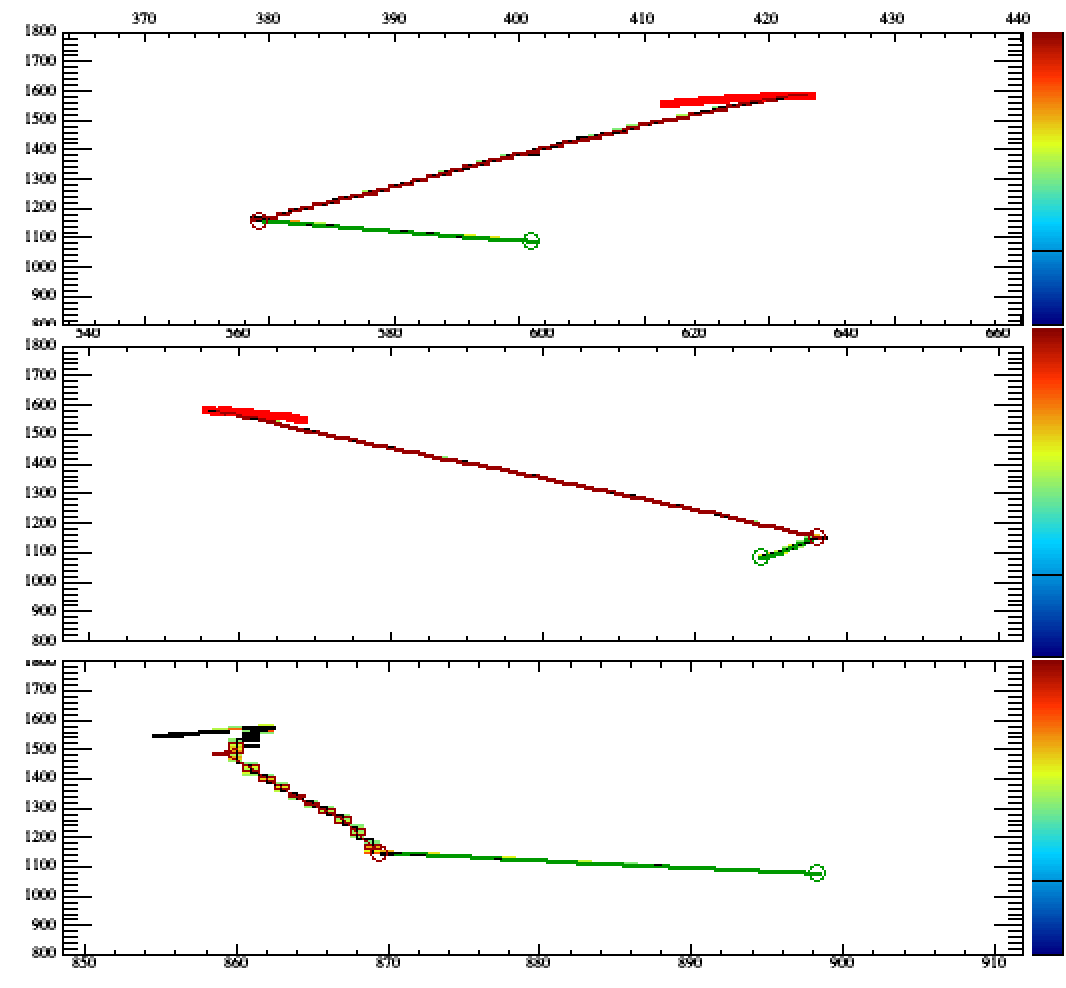
\includegraphics[width=0.8\textwidth]{event_signal.png}
\end{dunefigure} 

\begin{dunefigure}
[$p\rightarrow K^{+} \bar{\nu}$ background event displays]{fig:event_bkgd}
{Event displays for $p\rightarrow K^{+} \bar{\nu}$ backgrounds.  The vertical axis is time ticks (each time tick corresponds to 500 ns), and the horizontal axis is wire number. The bottom view is induction plane 1, middle is induction plane 2 and top is the collection plane. The color represents the charge deposited in each hit. The left shows an atmospheric neutrino interaction unlikely to be classified as signal. The right shows an atmospheric neutrino interaction which could make it into the selected sample without a tight cut.}
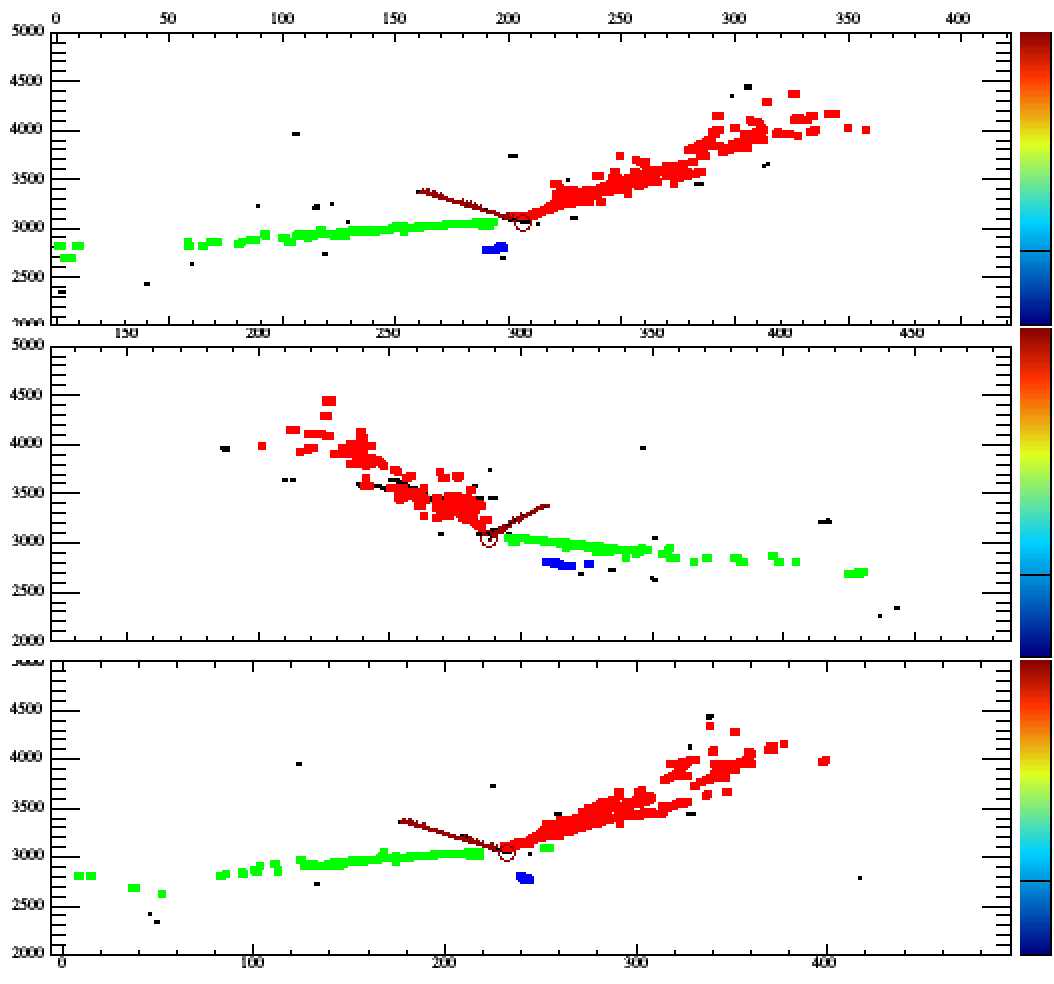
\includegraphics[width=0.48\textwidth]{event_bkgd_1.png}
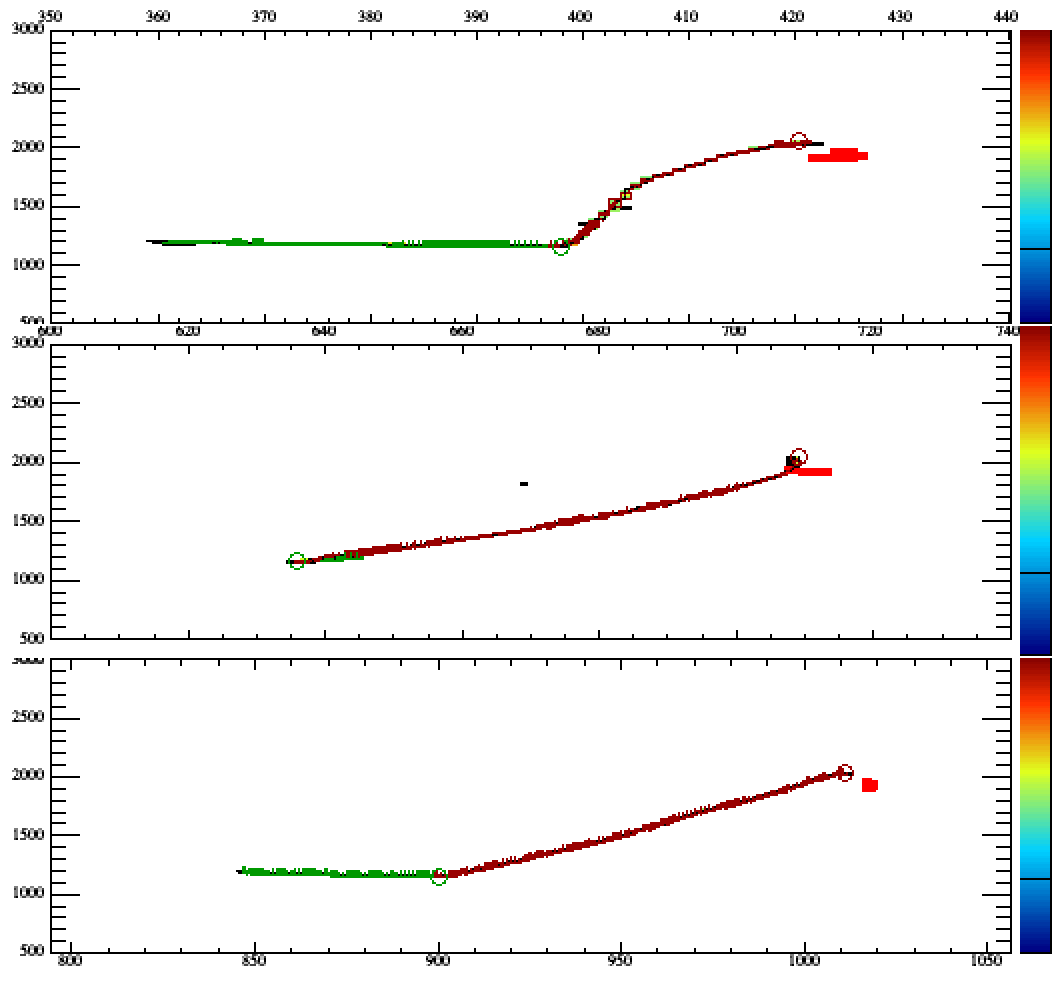
\includegraphics[width=0.48\textwidth]{event_bkgd_2.png}
\end{dunefigure}

Optimal lifetime sensitivity is achieved by combining the pre-selection cuts with a \dword{bdt} cut that gives a signal efficiency of 0.15 and a background efficiency of $3\times 10^{-6}$, which corresponds to approximately 1 background event per Mton-year. Assuming no signal is observed over 10 years of running with a total of 40~kton of fiducial mass, a 90$\%$ \dword{cl} upper limit on the proton lifetime in this channel of $6.6\times10^{33}$~years can be set. This calculation assumes constant signal and background efficiency over time and for each of the far detector modules.  Additional running improves the sensitivity proportionately if the experiment remains background-free.

The dominant systematic uncertainty in the signal is expected to be due to the kaon \dword{fsi}. To account for this uncertainty, kaon-nucleon elastic scattering ($K^{+}p(n)\rightarrow K^{+}p(n)$) is re-weighted by $\pm 50\%$ in the simulation. The spread in signal efficiency with this re-weighting is $(15\pm 2)\%$, which is taken as the  systematic uncertainty on the signal efficiency.
The dominant uncertainty in the background 
is due to the absolute normalization of the atmospheric neutrino rate. The Bartol group has carried out a detailed study of the systematic uncertainties, where the absolute neutrino fluxes have uncertainties of approximately 15$\%$~\cite{Barr:2006it}.
The remaining uncertainties are due to the cross section models for neutrino interactions. Uncertainty in the total $\nu$ \dword{cc} cross section peaks at 8$\%$ in the 1-5 GeV region~\cite{Adamson:2012gt}.
Based on these two effects, a conservative 20$\%$ systematic uncertainty in the background is estimated.
%Finally a 0.1$\%$ uncertainty in the calculation of the fiducial volume is proposed. 

The limiting factor in the sensitivity is the kaon tracking efficiency.  With the current reconstruction, 
%the tracking efficiency for kaons plateaus at approximately 80\% for high-energy kaons.  However, after \dword{fsi}, many kaons have energy less than 40 MeV, below the tracking threshold, leading to 
the overall kaon tracking efficiency is 58\%.
A visual scanning exercise indicates that the kaon tracking efficiency could be improved to approximately 80\%, where the remaining inefficiency comes from kaons that charge exchange, scatter, or decay in flight.
%Studies show that if all kaons with a path length of 2~cm or longer could be tracked (excluding kaons that decay in flight), tracking efficiency could improve to approximately 80\%.  
Combining this tracking performance improvement with some improvement in the $K/p$ separation performance for short tracks, the overall signal selection efficiency could improve from 15\% to approximately 30\%.  This would double the sensitivity.  

\subsection{Sensitivity to Other Key Nucleon Decay Modes}
\label{subsec:nonaccel-ndk-other}

Another potential mode for a baryon number violation search is the decay of the neutron into a charged lepton plus meson, i.e.~$n\rightarrow e^{-}K^{+}$. The current best limit on this mode is $3.2\times 10^{31}$~years from the FREJUS collaboration~\cite{Berger:1991fa}. The reconstruction software for this analysis is the same as for the $p\rightarrow \bar{\nu} K^{+} $ analysis; the analysis again uses a \dword{bdt} that includes image classification score as an input. To calculate the lifetime sensitivity for this decay mode the same systematic uncertainties and procedure is used. The final selection efficiency for this channel is 0.23, with a background efficiency of 5$\times 10^{-5}$, which corresponds to 15 background events per Mton-year. The lifetime sensitivity for a 400~kton$\cdot$year exposure is 5.4$\times 10^{33}$~years. As in the $p\rightarrow \bar{\nu}K^{+}$ analysis, challenges come from kaon \dword{fsi} and reconstruction; tracking and particle identification could be improved, so efficiency and thus the lifetime sensitivity could be doubled.  Nevertheless, with the current reconstruction and analysis tools, the DUNE \dword{fd} technology can improve the lifetime limit for this particular channel by two orders of magnitude.

The sensitivity to the $p \rightarrow e^{+} \pi^0$ mode has also been calculated. For this analysis, reconstruction was not applied, and true quantities were used as inputs to a \dword{bdt} to isolate events that contain a positron and two photons from the $\pi^0$ decay.  Energy smearing simulated the effects of reconstruction.  Applying the same selection to the atmospheric neutrino background and calculating the limit yields a sensitivity for an exposure of 800~kton-years in the range of $1.2 \times 10^{34}$ to $1.5 \times 10^{34}$~years depending on the level of energy smearing (in the range 5-30\%).  This analysis is preliminary, but it indicates that DUNE could achieve a sensitivity comparable to \superk's current limit of $1.6 \times 10^{34}$~years~\cite{Miura:2016krn}.

\subsection{Detector Requirements for Nucleon Decay Searches}
\label{subsec:nonaccel-ndk-requirements}

As is the case for the entire far detector non-accelerator 
based physics program of DUNE, nucleon decay searches require 
efficient triggering and event localization  
capabilities. The nucleon decay search program also relies 
on both the event imaging and particle identification 
(via dE/dx) capabilities of the \lartpc technology.  

Event localization within the far detector along the ionization 
drift direction is required in order to reject cosmic ray 
backgrounds via fiducial volume cuts. This can be achieved by 
requiring an event time ($T0$) signal for nucleon decay 
candidates so that TPC anode signal times can be used to 
determine the drift time.  Within DUNE, the $T0$ is provided by 
the photon detection system, which must have high detection 
efficiency throughout the far detector active volume for a 
scintillation photon signal corresponding to 
$>\SI{100}{\MeV}$ of deposited energy.

%\todo{Discussion of using timing to demonstrate that the signals from kaon decay products are delayed with respect to those from the kaon track itself, consistent with kaon lifetime. }
For nucleon decays into charged kaons, the possibility of using 
the time difference between the kaon scintillation signal and 
the scintillation signal from the muon from the kaon decay has 
been investigated.  
In the \superk analysis of $p\to\bar{\nu} K^{+}$, the 
corresponding timing difference (between the de-excitation 
photons from the oxygen nucleus and the muon from kaon decay) 
was found to be an effective way to reduce
backgrounds~\cite{Abe:2014mwa}.  
Studies indicate that measuring time differences on the scale 
of the kaon lifetime (\SI{12}{\ns}) is difficult in DUNE, 
independent of photon detector acceptance and timing resolution, 
due to both the scintillation process in argon 
-- consisting of fast (\si{\ns}-scale) and slow (\si{\micro\second}-scale) components --  and 
Rayleigh scattering over long distances.

Given the $\sim \SI{1}{GeV}$ energy release, 
the requirements for tracking 
and calorimetry performance are similar to those for the 
beam-based neutrino oscillation program described 
in Chapter~\ref{ch:osc}.  Especially important are the 
event imaging function and and the $dE/dx$ measurement 
capability for particle identification.   
With a well-functioning \lartpc, nucleon decay search  
capabilities are ultimately limited by physics, namely
complexities arising from 
final state interactions (such as nucleon emission) 
as well as ionization fluctuations for example, 
rather than by detector performance {\sl per se}. This is 
the case provided that readout noise is small compared to 
the ionization signal expected for minimum-ionizing particles
located anywhere within the active volume of the detector 
(see Sec.~\ref{sec:exec-key-reqs}).
%However, degradation of detector performance relative to 
%specifications for some combination of drift field, 
%electron lifetime and system noise 
%(see Sec.~\ref{ch-exec-key-reqs}) would impact the 
%sensitivity of the nucleon decay program.



%Experimental challenges, such as particle identification to separate protons from kaons, 
%the impact of \dword{fsi} on proton decay kinematics, and full control
%of the potential background processes, are under study with realistic detector simulations.
%This includes opportunities for enhanced background rejection using \dword{cnn}s and efforts to understand the
%uncertainty associated with the intra-nuclear cascade model used to simulate \dword{fsi}. 
%%Especially critical is the exquisite $dE/dx$ resolution offered by the \lartpc response. 
%\dword{protodune} data taken with charged particle beams at CERN should 
%provide an important sample of events to train and improve reconstruction algorithms and the resulting $dE/dx$ resolution.

\subsection{Nucleon Decay Summary}
\label{sec:ndksummary}

In summary, an analysis of DUNE's sensitivity to proton decay via $p\rightarrow K^{+} \bar{\nu}$ with full simulation and reconstruction shows that the sensitivity after a 400~kton$\cdot$years exposure
is comparable to the current limit from \superk based on an exposure of 260~kton$\cdot$years.  Previous estimates of the sensitivity in this channel in a \lartpc~\cite{Acciarri:2015uup} did not consider kaon \dword{fsi} and were overly optimistic about the kaon tracking efficiency, assuming a nearly perfect signal detection efficiency.  An analysis of the sensitivity to neutron decay via $n\rightarrow e^{-}K^{+}$ has also been completed; DUNE could improve the lifetime limits in this mode by two orders of magnitude.  Future studies of nucleon decay into kaons will focus on potential improvements in track reconstruction, improved methods of particle and event identification, and understanding kaon \dword{fsi} models.  Studies indicate improvements in these areas could double the sensitivity to these modes. 
%Figure~\ref{fig:sens} summarizes the sensitivity of the two kaon modes studied so far. 
Analysis of other modes of proton decay into kaons is underway, as well as the first investigations of the $p \rightarrow e^{+}\pi^0$ with full simulation and reconstruction.

%\begin{dunefigure}
%[Kaon mode sensitivity]{fig:sens}
%{DUNE's sensitivity for two modes of nucleon decay to charged kaons for a 400 kton-year exposure, with the current reconstruction and with potential improvements.  The current lifetime limits for these two modes~\cite{Abe:2014mwa,Berger:1991fa} are also shown.}
%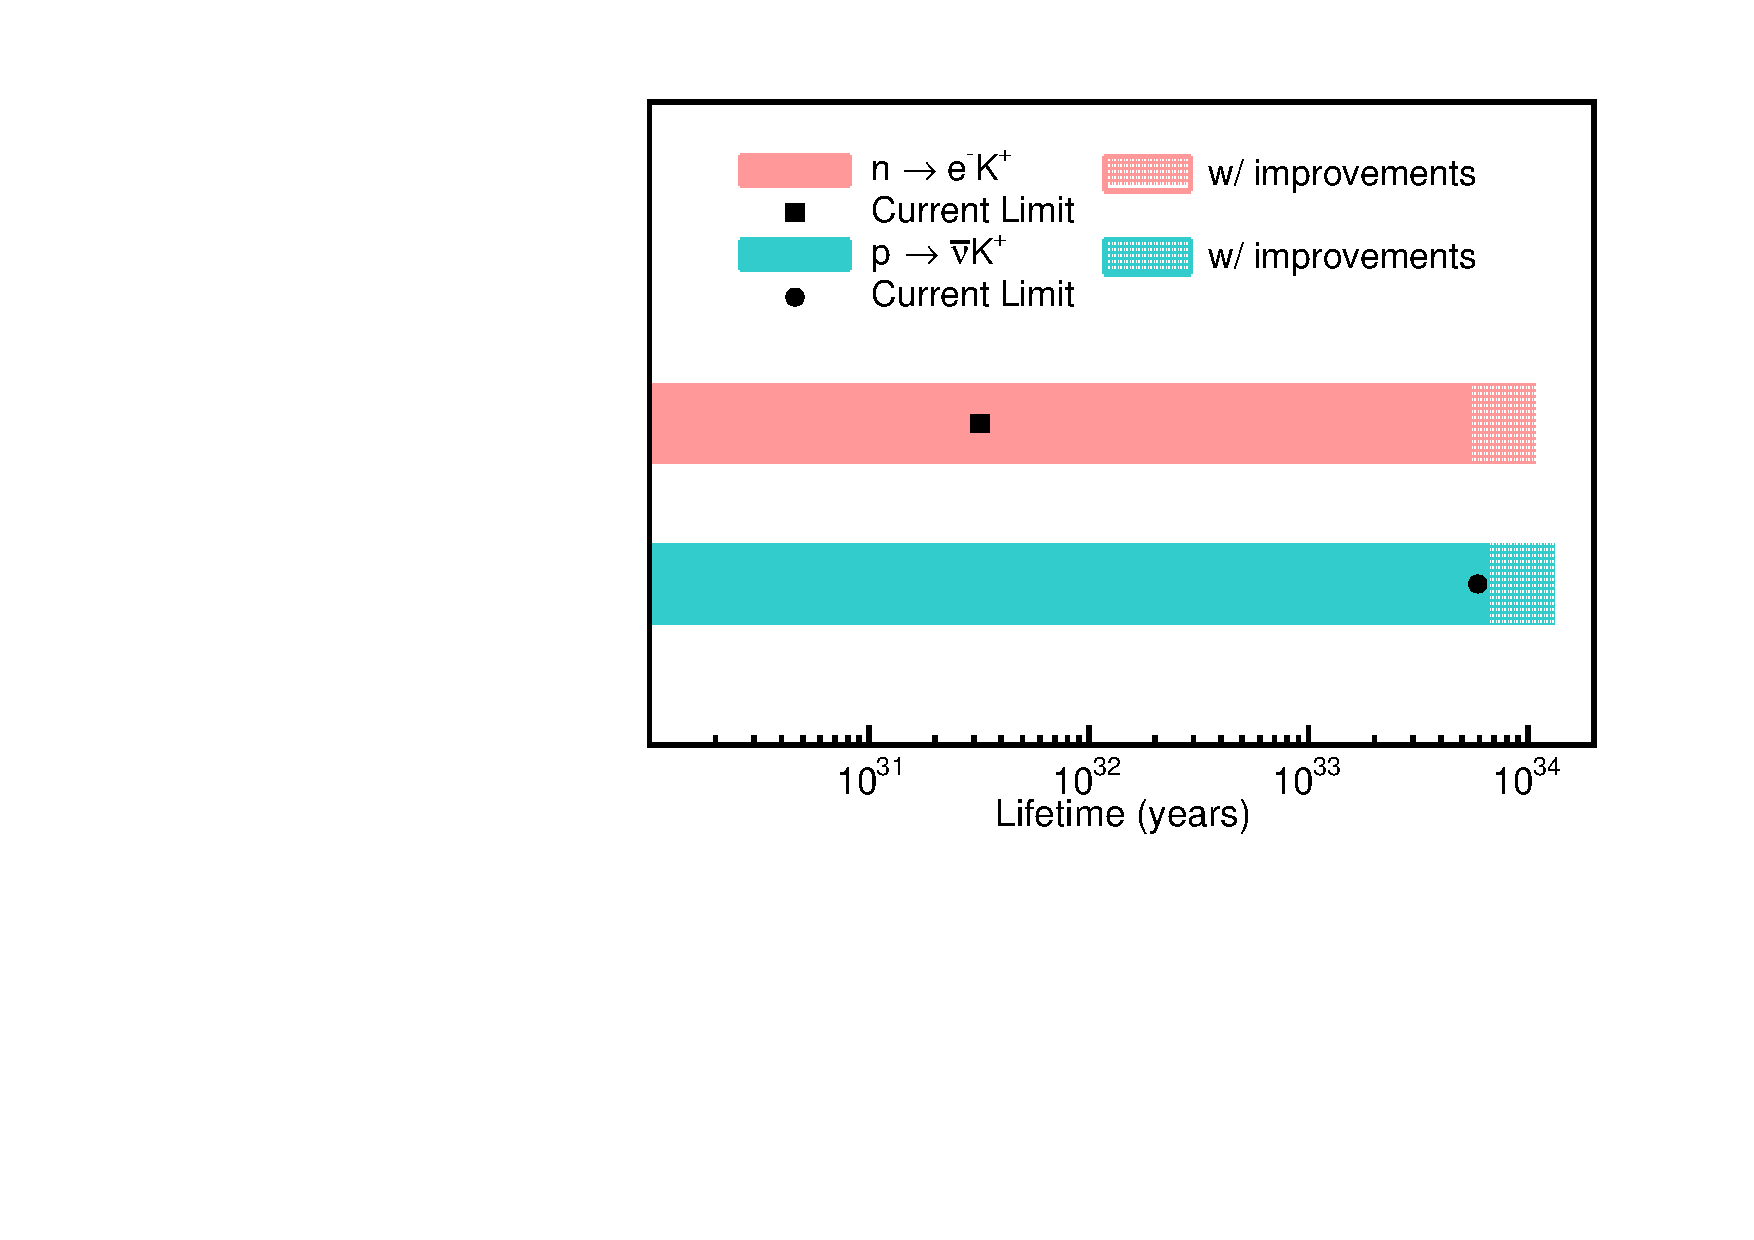
\includegraphics[width=0.8\textwidth]{sens.pdf}
%\end{dunefigure} 


%%%%%%%%%%%%%%%%%%%%%%%%%%%%%%%%%%%%%%%%%%%%%%%%%%%%%%%%%%%%%%%%
\section{N-Nbar Oscillations}
\label{sec:nonaccel-nnbar}

%\fixme{Section 1.2.1 appears to be background to the entire section and could serve as an introduction to the section under the major heading N-Nbar Oscillations. This would change the numbering but would also provide that introduction.}

%\subsection{Motivation for $\Delta$B=2 Physics and Possible Experimental Approaches}
%\label{subsec:nonaccel-nnbar-intro}

Neutron-antineutron ($n - \bar{n}$) oscillation is a baryon number violating process that
has never been observed but is predicted by a number of Beyond Standard Model
theories~\cite{Phillips:2014fgb}. In this context, baryon number conservation is an accidental
symmetry rather than a fundamental one, which means baryon number violation
does not stand against the fundamental gauge symmetries. Discovering baryon
number violation would have implications about the source of matter-antimatter
symmetry in our universe given Sakharov's conditions for such asymmetry to arise~\cite{Sakharov:1967dj}.
In particular, the neutron-antineutron oscillation ($n-\bar{n}$ or n-nbar) process violates
baryon number by two units and, therefore, could also have further implications for
the smallness of neutrino masses~\cite{Phillips:2014fgb}. The $n - \bar{n}$ process is one of many possible baryon number violating processes that DUNE can search for. Searches for this process using
both free neutrons and nucleus-bound neutron states have continued 
since the 1980s. The current best 90\% \dword{cl} limits on the (free) neutron oscillation
lifetime from free n-nbar searches is $8.6\times10^7$~s and from nucleus-bound n-nbar searches is $2.7\times 10^8$~s~\cite{BaldoCeolin:1994jz,Abe:2011ky}.

Neutron-antineutron oscillations can be detected via the subsequent antineutron annihilation with a neutron or a proton. Table~\ref{tab:nnbar-br} shows the branching ratios for the antineutron annihilation modes applicable to intranuclear searches.  This annihilation event will have a distinct signature of a vertex with several emitted light hadrons, with total energy of twice the nucleon mass and zero net momentum. Reconstructing these hadrons correctly and measuring their energies is key to identifying the signal event. The main background for these $n - \bar{n}$ annihilation events is caused by atmospheric neutrinos. Most common among mis-classified events are neutral current deep inelastic scattering events without a lepton in the final state. As with nucleon decay, nuclear effects and final state interactions make the picture more complicated.


\begin{table}
\caption[n-nbar annihiliation modes]{Effective branching ratios for antineutron annihilation in $^{40}$Ar, as implemented
in GENIE.}
\begin{tabular}{p{.22\textwidth}p{.22\textwidth}p{.22\textwidth}p{.22\textwidth}}
\rowcolor{dunetablecolor} 
\multicolumn{2}{^c}{$\bar{n}+p$} & \multicolumn{2}{^c}{$\bar{n}+n$}\\
\rowcolor{dunetablecolor}
         Channel & Branching ratio & Channel & Branching ratio \\ \toprowrule
         $\pi^{+}\pi^{0}$ & 1.2\% & $\pi^{+}\pi^{-}$ & 2.0\% \\ \colhline
         $\pi^{+}2\pi^{0}$ & 9.5\% & $2\pi^{0}$ & 1.5\% \\ \colhline
         $\pi^{+}3\pi^{0}$ & 11.9\% & $\pi^{+}\pi^{-}\pi^{0}$ & 6.5\% \\ \colhline
         $2\pi^{+}\pi^{-}\pi^{0}$ & 26.2\% & $\pi^{+}\pi^{-}2\pi^{0}$ & 11.0\% \\ \colhline
         $2\pi^{+}\pi^{-}2\pi^{0}$ & 42.8\% & $\pi^{+}\pi^{-}3\pi^{0}$ & 28.0\% \\ \colhline
         $2\pi^{+}\pi^{-}2\omega$ & 0.003\% & $2\pi^{+}2\pi^{-}$ & 7.1\% \\ \colhline
         $3\pi^{+}2\pi^{-}\pi^{0}$ & 8.4\% & $2\pi^{+}2\pi^{-}\pi^{0}$ & 24.0\% \\ \colhline
          &  & $\pi^{+}\pi^{-}\omega$ & 10.0\% \\ \colhline
          &  & $2\pi^{+}2\pi^{-}2\pi^{0}$ & 10.0\% \\ \colhline
\label{tab:nnbar-br}
\end{tabular}
\end{table}



\subsection{Sensitivity to Intranuclear Neutron-Antineutron Oscillations in DUNE}
\label{subsec:nonaccel-nnbar-dunesensitivity}

The simulation of neutron-antineutron oscillation was developed~\cite{Hewes:2017xtr} and implemented in GENIE. This analysis uses GENIE v.2.12.10.
%(see Table~\ref{tab:genie-antineutron} in Appendix~\ref{sec:tools-app-generator} for a list of interaction channels available in \dword{genie}).  
Implementing this process in GENIE used GENIE's existing modeling of Fermi momentum and binding energy for both the oscillating neutron and the nucleon with which the resulting antineutron annihilates.   Once a neutron has oscillated to an antineutron in a nucleus, the antineutron has a 18/39 chance of annihilating with a proton in argon, and a 21/39 chance of annihilating with a neutron. The energies and momenta of the annihilation products are assigned randomly but consistently with four-momentum conservation. The products of the annihilation process follow the branching fractions (shown in Table~\ref{tab:nnbar-br}) measured in low-energy antiproton annihilation on hydrogen.
%, biased as necessary by conservation of total available energy in the annihilation \textcolor{red}{the last part is not clear}. 
Since the annihilation products are produced inside the nucleus, GENIE further models re-interactions of those products as they propagate in the nucleus (until they escape the nucleus).  The \dword{fsi} are simulated using the $hA2015$ model in GENIE as described in Section~\ref{sec:final-state-interactions}.

Figure \ref{fig:pi_FSI_m} shows the momentum distributions for charged and neutral pions before \dword{fsi} and after \dword{fsi}. These distributions show the \dword{fsi} makes both charged and neutral pions less energetic.  The effect of \dword{fsi} on pion multiplicity is also rather significant; 0.9$\%$ of the events have no charged pions before \dword{fsi}, whereas after \dword{fsi} 11.1$\%$ of the events have no charged pions. In the case of the neutral pion, 11.0 $\%$ of the events have no neutral pions before \dword{fsi}, whereas after \dword{fsi}, 23.4$\%$ of the events have no neutral pions. The decrease in pion multiplicity is primarily due to pion absorption in the nucleus. Another effect of \dword{fsi} is nucleon knockout from pion elastic scattering. Of the events, 94$\%$ have at least one proton from \dword{fsi} and 95$\%$ of the events have at least one neutron from \dword{fsi}. Although the kinetic energy for these nucleons peak at a few tens of MeV, the kinetic energy can be as large as hundreds of MeV.  In summary, the effects of \dword{fsi} in $n-\bar{n}$ become relevant because they modify the kinematics and topology of the event. For instance, even though the decay modes of Table \ref{tab:nnbar-br} do not include nucleons in their decay products, nucleons appear with high probability after \dword{fsi}.

\begin{dunefigure}
[FSI in n-nbar]{fig:pi_FSI_m}
{Momentum of an individual charged pion before and after final state interactions (left): momentum of an individual neutral pion before and after final state interactions (right).}
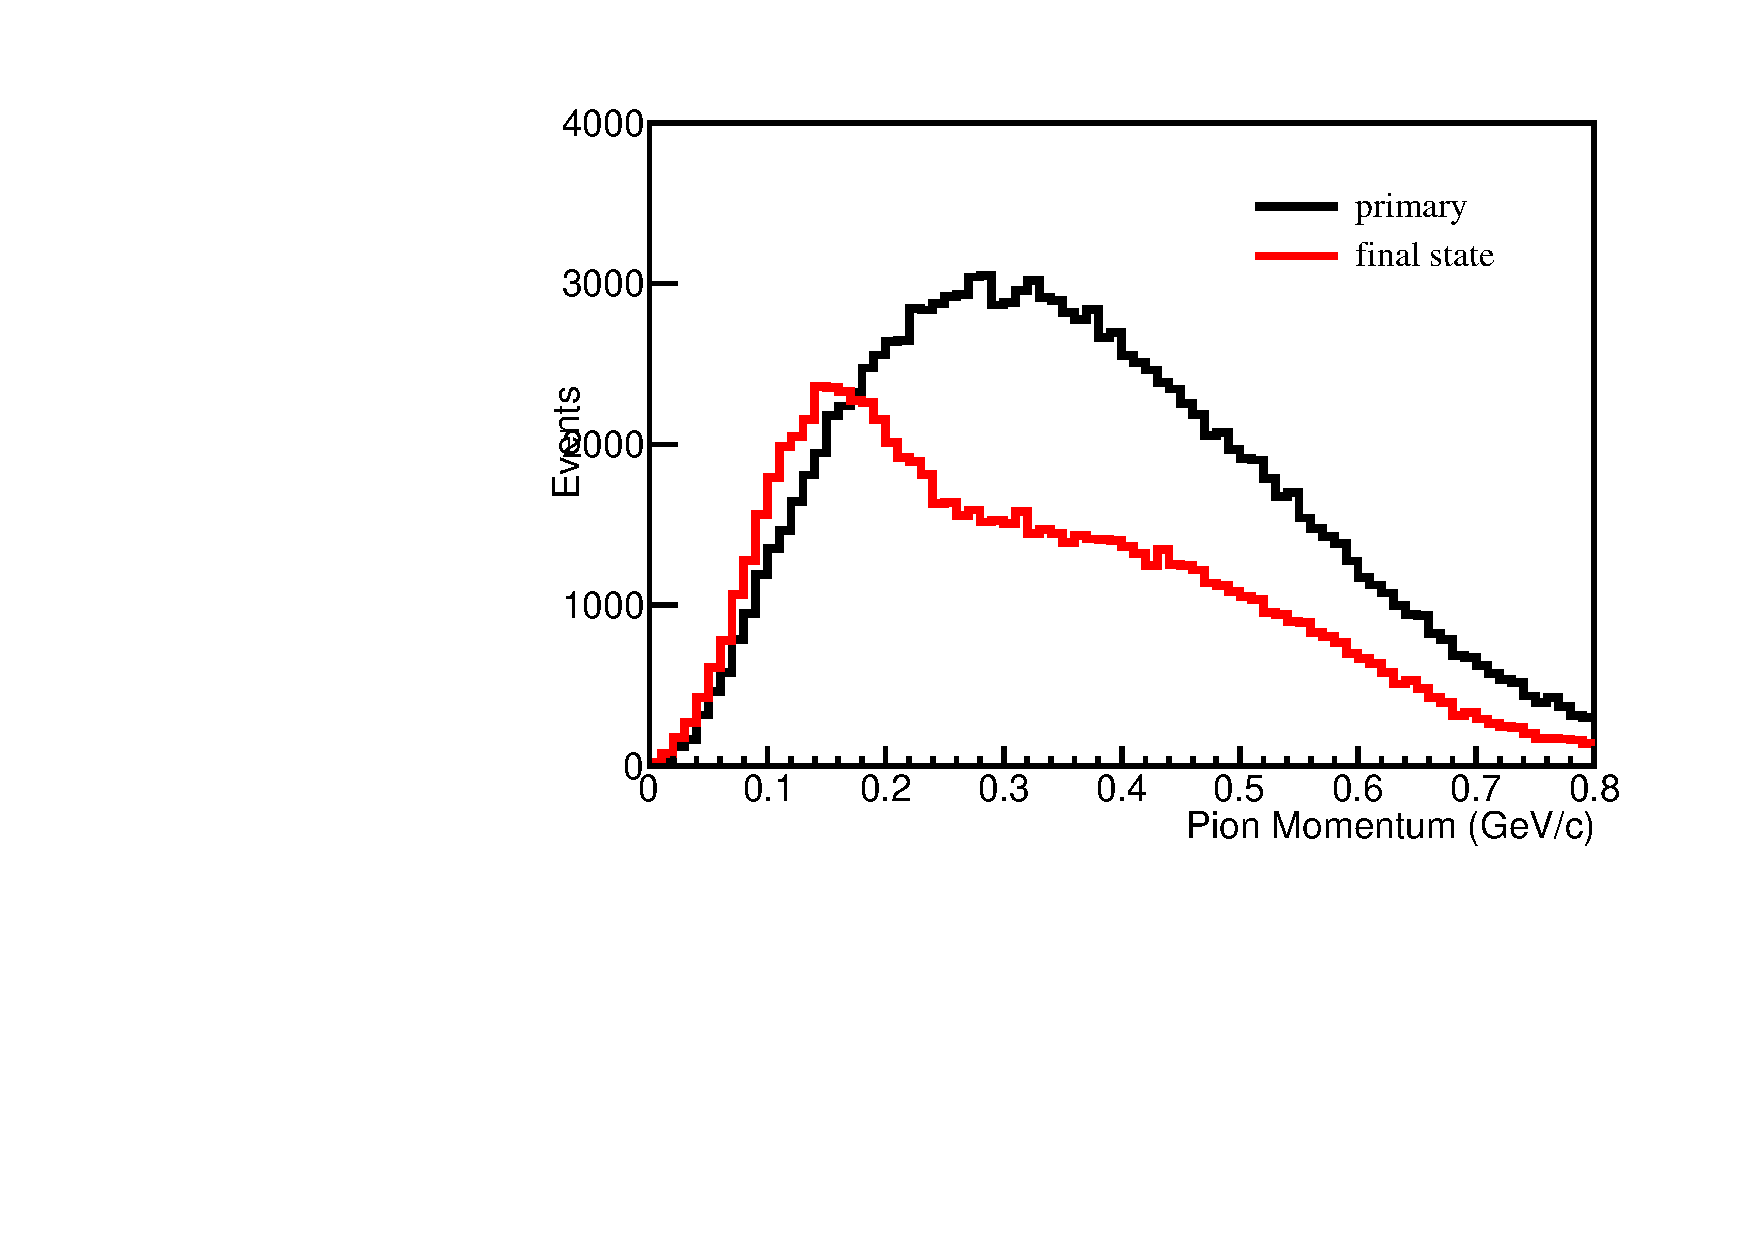
\includegraphics[width=0.49\textwidth]{pi_mom.pdf}
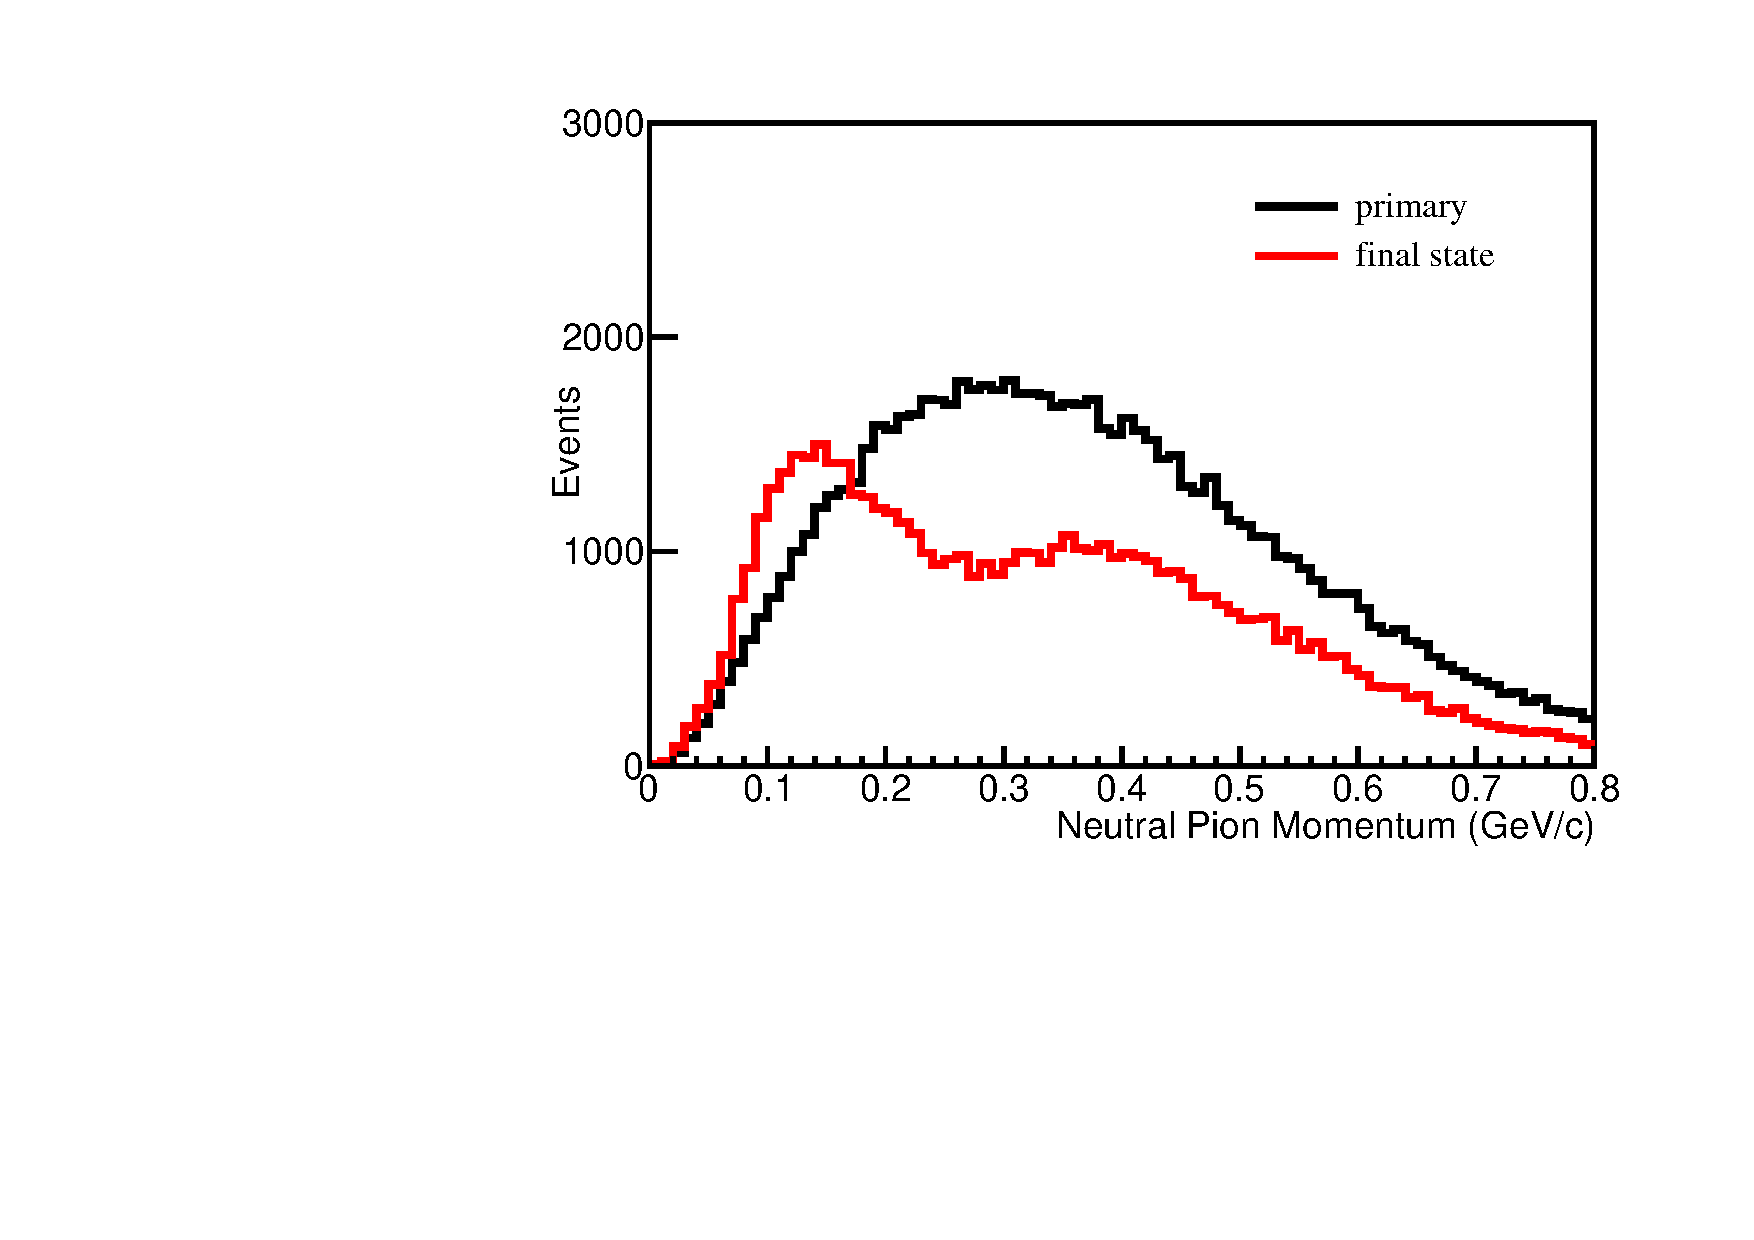
\includegraphics[width=0.49\textwidth]{pizero_mom.pdf}
\end{dunefigure} 

The main background process in search of bound $n-\bar{n}$ oscillation in DUNE is assumed to be atmospheric neutrino interactions in the detector.  This is simulated in GENIE as described in Section~\ref{sec:ndkbkgd}.

As with the $p\rightarrow K^{+} \bar{\nu}$ analysis, two distinct methods of reconstruction and event selection have been applied in this search. One involves traditional reconstruction methods (\threed track and vertex reconstruction by \dword{pma}); 
%\fixme{PMA is not in the glossary.} 
the other involves image classification 
%on TPC \twod projections of TPC collection plane wires vs. drift distance (CNN). 
of \twod images of reconstructed hits. The two methods, combined in the form of a multivariate analysis, uses the image classification score with other physical observables extracted from traditional reconstruction.  A \dword{bdt} classifier is used. Ten variables are used in the \dword{bdt} event selection, including number of reconstructed tracks and showers; variables related to visible energy deposition; $PIDA$ and $dE/dx$; reconstructed momentum; and CNN score.  Figure~\ref{fig:bdt_nnbar} shows the distribution of the \dword{bdt} output for signal and background.

\begin{dunefigure}
[n-nbar BDT response]{fig:bdt_nnbar}
{Boosted Decision Tree response for $n-\bar{n}$ oscillation for signal (blue) and background (red).}
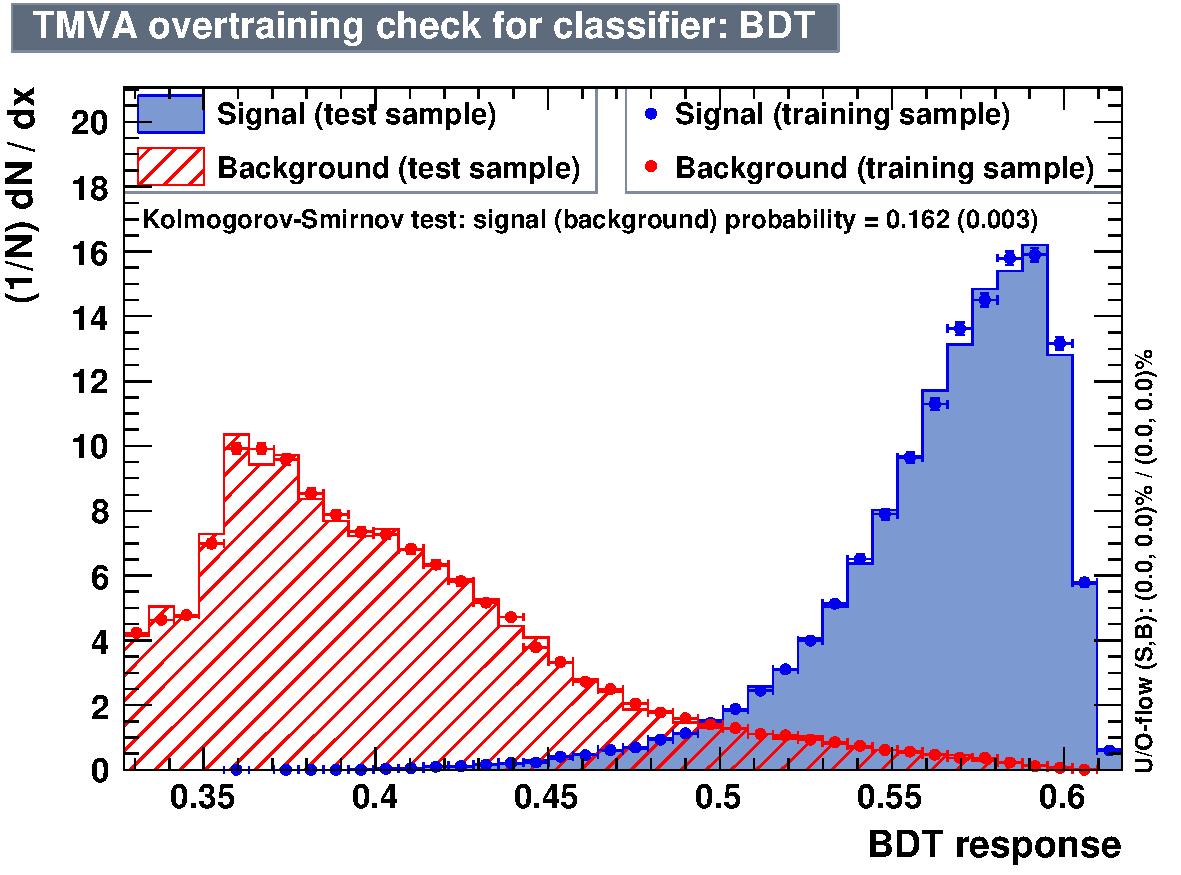
\includegraphics[width=0.8\textwidth]{BDT_nnbar.pdf}
\end{dunefigure} 

%\begin{dunefigure}
%[Efficiency of BDT selection]{fig:BDT_nnbar_eff}
%{BDT selection efficiency for n-nbar signal and background.}
%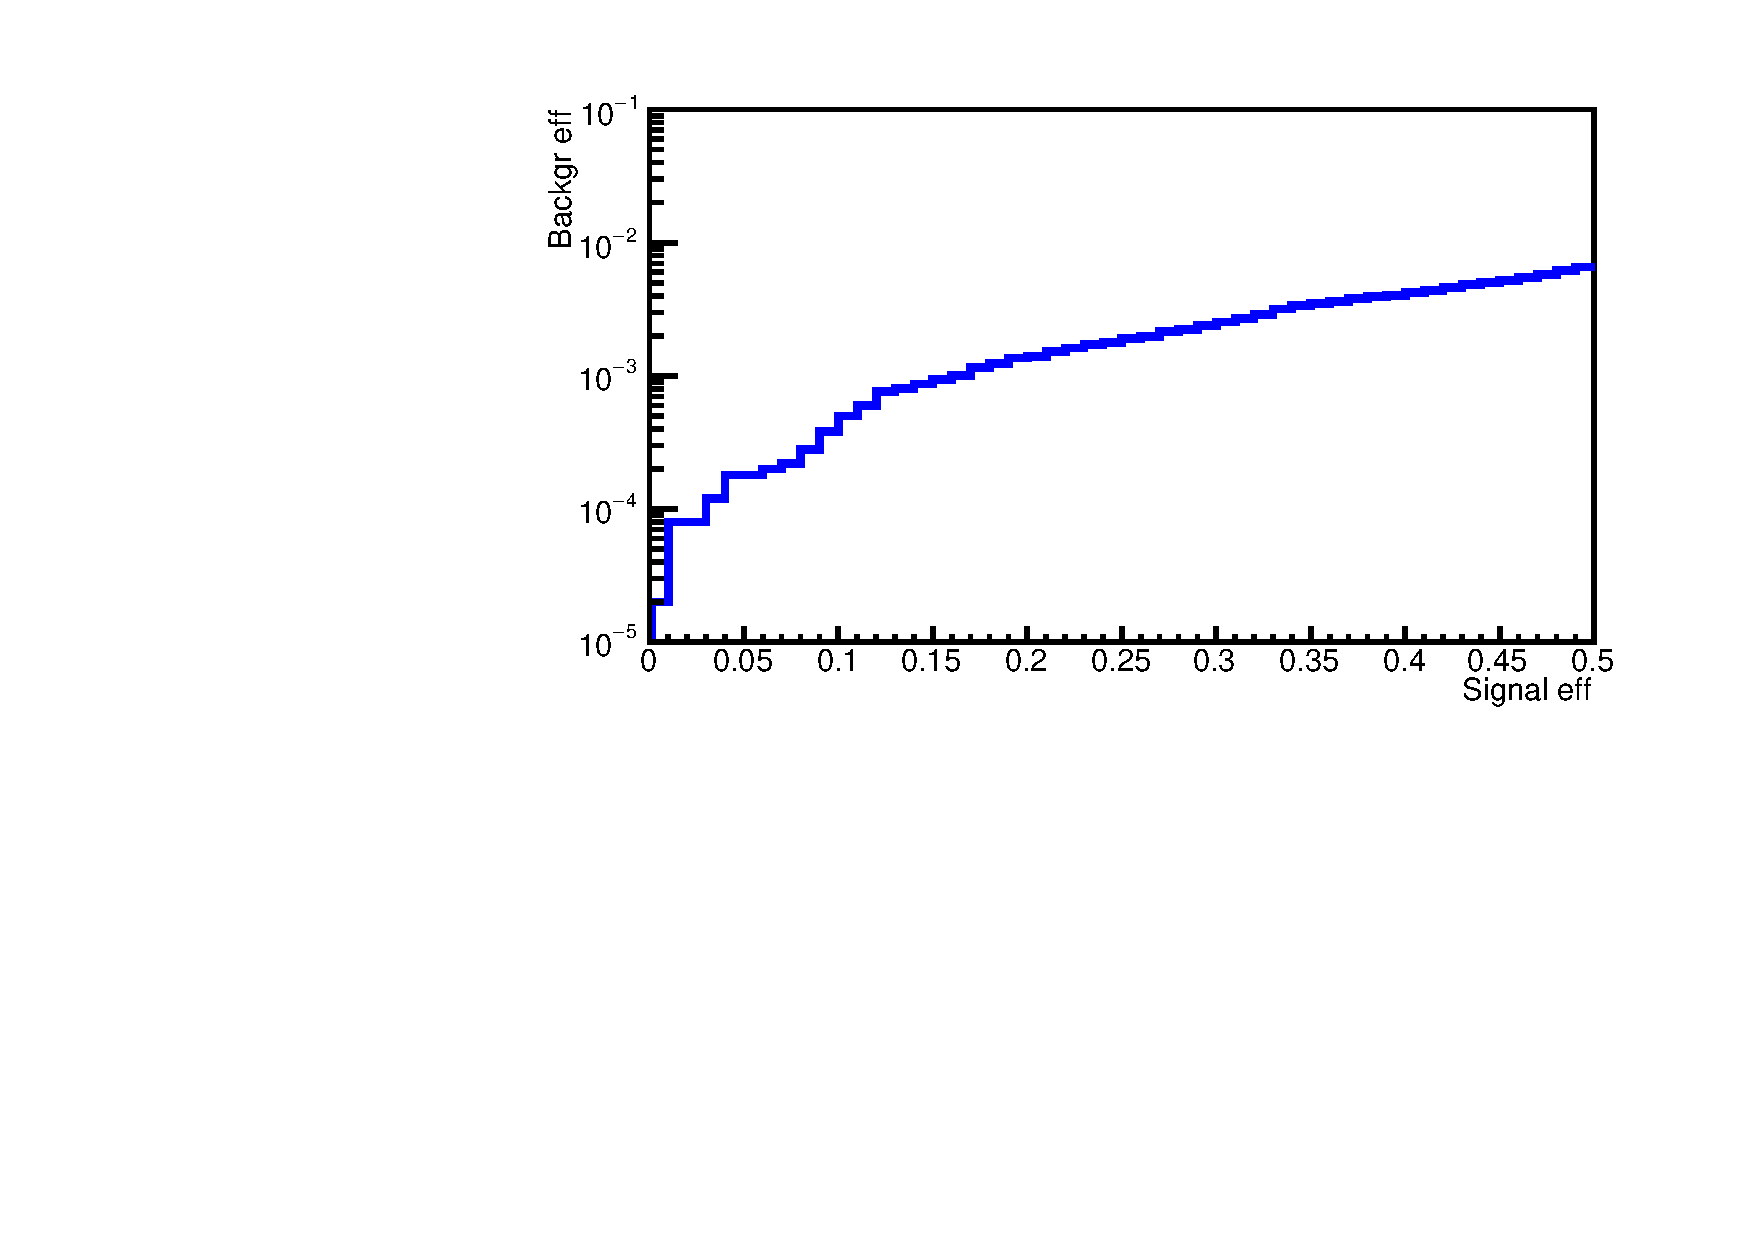
\includegraphics[width=0.8\textwidth]{BDT_nnbar_eff.pdf}
%\end{dunefigure} 

Figure \ref{fig:nnbar_sig} shows an $n-\bar{n}$ event with high \dword{bdt} response value (0.592). Showers from neutral pions are shown in red, blue, yellow, and green. The reconstructed charged pion tracks are shown as green and maroon lines. The topology of this event is consistent with charged pion and neutral pion production. 

The left side plot in Figure \ref{fig:nnbar_bkgd} shows a \dword{nc} background event $\nu_{e}+n\rightarrow \nu_{e}+p+p$ with a low \dword{bdt} response value (0.388). The two protons from the \dword{nc} interaction are reconstructed as tracks, and no shower activity is present. The right side plot in Figure \ref{fig:nnbar_bkgd} displays a \dword{cc} background event $\nu_{e}+n\rightarrow {e}^{-}+p+\pi +p$ with a high \dword{bdt} response value (0.598). This background event mimics the signal topology by having multi-particle production and an electromagnetic shower. Further improvements in shower reconstruction, especially $dE/dx$, should help in classifying these types of background events in the future because the electron shower $dE/dx$ differs from the $dE/dx$ of a shower induced by a gamma-ray.

\begin{dunefigure}
[Event display for well-classified n-nbar signal event]{fig:nnbar_sig}
{Event display for a well-classified n-nbar signal event.  The vertical axis is time ticks (each time tick corresponds to 500 ns), and the horizontal axis is wire number.  The bottom view is induction plane 1, middle is induction plane 2, and the top is the collection plane.  The color represents the charge deposited in each hit.}
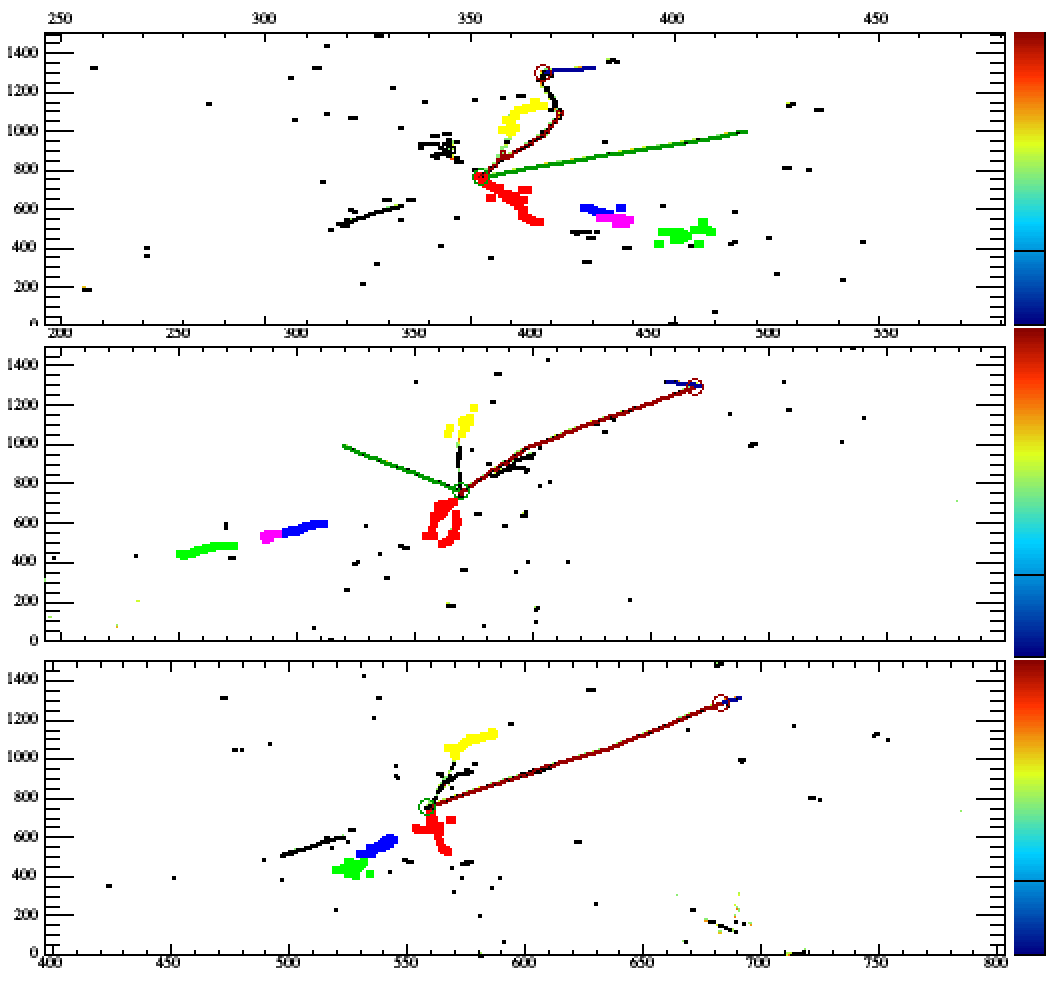
\includegraphics[width=0.8\textwidth]{nnbar_sig.png}
\end{dunefigure} 

%\fixme{In the figure title, an abbreviation is used (ADC). According to the glossary, this should be analog to digital converter. Is that correct? In that case the abbreviation should be spelled out for the figure title, while ADC in the text should use the dword code. This also applies to Figure 1.12. (A reminder here: BDT is not in the document glossary.)}

\begin{dunefigure}
[Event displays for n-nbar background events]{fig:nnbar_bkgd}
{Event displays for n-nbar backgrounds.  The vertical axis is time ticks (each time tick corresponds to 500 ns), and the horizontal axis is wire number.  The bottom view is induction plane 1, middle is induction plane 2, and the top is the collection plane.  The color represents the charge deposited in each hit.  The left plot shows an atmospheric neutrino interaction unlikely to be classified as signal. The right plot shows an atmospheric neutrino interaction which could make it into the selected sample.}
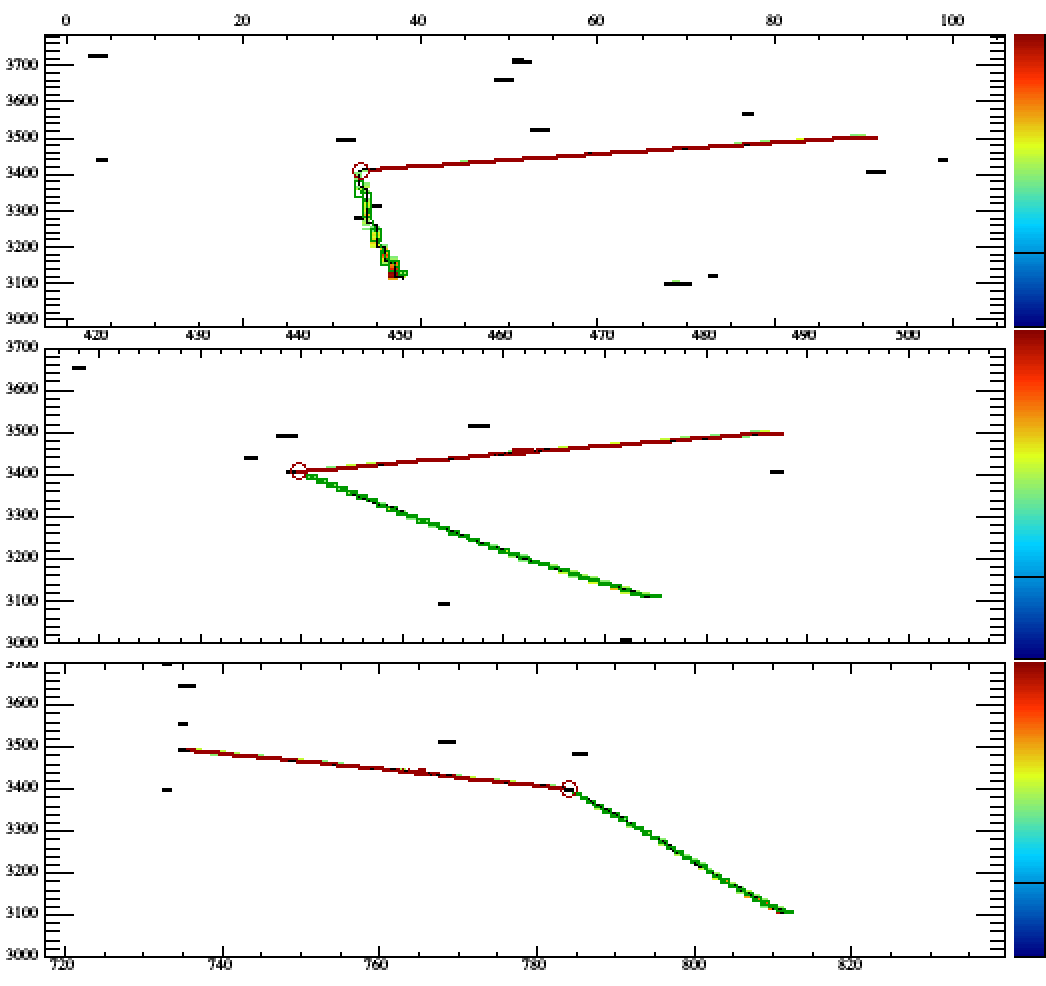
\includegraphics[width=0.49\textwidth]{nnbar_bkgd_ev2.png}
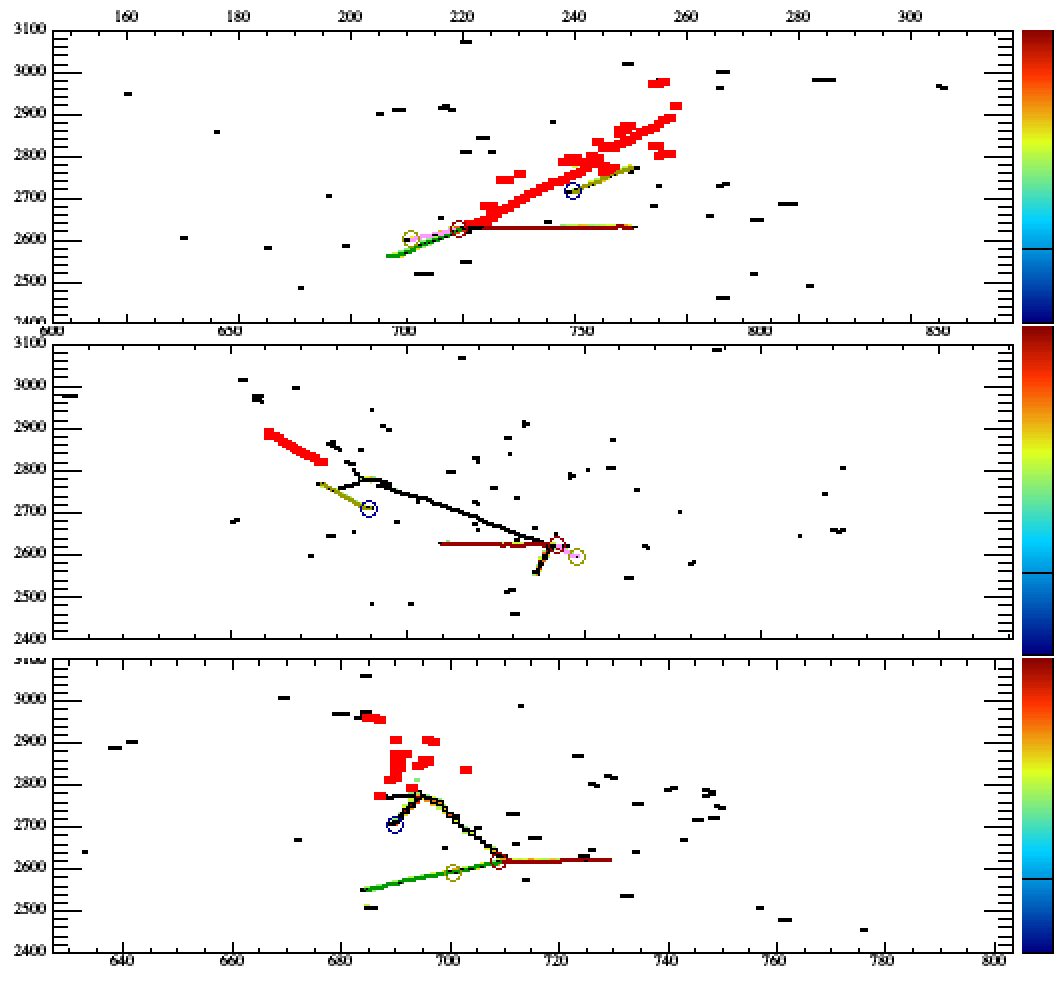
\includegraphics[width=0.49\textwidth]{nnbar_bkgd_ev1.png}
\end{dunefigure} 

The sensitivity to the $n-\bar{n}$ oscillation lifetime can be calculated for a given exposure, the efficiency of selecting signal events, and the background rate along their uncertainties. The lifetime sensitivity is obtained at 90\% \dword{cl} for the bound neutron. Then, the lifetime sensitivity for a free neutron is acquired using the conversion from nucleus bounded neutron to free neutron $n-\bar{n}$ oscillation~\cite{Friedman:2008es}.  The preliminary systematic uncertainties on exposure (3\%), signal efficiency (25\%), and background efficiency (25\%) are taken from the $n-\bar{n}$ oscillation search by the \superk collaboration~\cite{Abe:2011ky}.

The free $n-\bar{n}$ oscillation lifetime, $\tau_{n-\bar{n}}$, and bounded $n-\bar{n}$ oscillation lifetime, $T_{n-\bar{n}}$, are related to each other through the suppression factor $R$ as

\begin{equation}
    \tau^{2}_{n-\bar{n}} = \frac{T_{n-\bar{n}}}{R} ~.
    \label{eq:tau}
\end{equation}
The suppression factor $R$ varies for different nuclei. This suppression factor was calclulated for $^{16}$O and $^{56}$Fe~\cite{Friedman:2008es}. The $R$ for $^{56}$Fe, $0.666\times10^{23}$ $s^{-1}$, is used in this analysis for $^{40}$Ar nuclei.

The best bound neutron lifetime limit is achieved using a signal efficiency of 8.0$\%$ at the background rejection probability of 99.98$\%$. The 90$\%$ \dword{cl} limit of a bound neutron lifetime is 6.45$\times 10^{32}$ years for a 400~kton-year exposure. The corresponding  limit for the oscillation time of free neutrons is calculated to be 5.53$\times 10^{8}$~s. This is approximately an improvement by a factor of two from the current best limit \cite{Abe:2011ky}.  Planned improvements to this analysis include improved \dword{cnn} performance and better estimates of systematic uncertainties.

%%%%%%%%%%%%%%%%%%%%%%%%%%%%%%%%%%%%%%%%%%%%%%%%%%%%%%%%%%%%%%%%
\section{Physics with Atmospheric Neutrinos}
\label{sec:nonaccel-atm}

Atmospheric neutrinos are a unique tool for studying neutrino oscillations: the oscillated flux contains all flavors of neutrinos and antineutrinos, is very sensitive to matter effects and to both $\Delta m^2$ parameters, and covers a wide range of $L/E$. In principle, all oscillation parameters could be measured, with high
complementarity to measurements performed with a neutrino beam. In addition, atmospheric neutrinos are available all the time, in particular before the beam becomes operational. The DUNE \dword{fd}, with its large mass and the overburden to protect it from atmospheric muon background, is an ideal tool for these studies.  Given the strong overlap in event topology and energy scale with beam neutrino interactions, most requirements will necessarily be met by the far detector design. Additional requirements include a self-trigger because atmospheric neutrino events are asynchronous with accelerator timing and thus a more stringent demand on neutrino direction reconstruction.

\subsection{Oscillation Physics with Atmospheric Neutrinos}
\label{sec:nonaccel-atm-oscillations}

Sensitivity to oscillation parameters with atmospheric neutrinos in DUNE has been evaluated.
%with a 
%dedicated simulation, reconstruction and analysis chain. 
The fluxes of each neutrino species were computed at the far detector location, after 
oscillation. Interactions in the \dword{lar} medium were simulated with the GENIE event 
generator. Detection thresholds and energy resolutions based on full 
simulations were applied to the outgoing particles to take 
detector effects into account. Events were classified as fully contained 
%\fixme{Fully contained should not be abbreviated. The glossary already uses FC for field cage.}
or partly contained
%\fixme{If fully contained is not abbreviated, then partly contained should not be. Many abbreviations already have "PC" in them.} 
by placing the vertex at a random position inside the 
detector and tracking the lepton until it reaches the edge of the detector. %its edges.  
Partly contained events 
are those where a final state muon exits the detector.  The number of events expected 
for each flavor and category is summarized in Table~\ref{tab:atmos_rates}.

\begin{dunetable}
[Atmospheric neutrino event rates]
{lc}
{tab:atmos_rates}
{Atmospheric neutrino event rates per year including oscillations in 40 kt of fiducial mass %\fixme{Spell out the abbreviations in figure/table titles.}
}
Sample   &  Event rate per year \\ \toprowrule
fully contained electron-like   & $1.6\times10^3$ \\ \colhline
fully contained muon-like       & $2.4\times10^3$ \\ \colhline
partly contained muon-like   & $7.9\times10^2$ \\ 
\end{dunetable}

%\begin{dunetable}
%[Atmospheric neutrino event rates]
%{lc}
%{tab:atmos_rates_old}
%{Atmospheric neutrino event rates including oscillations in \SI{350}{\ktyr}}
%Sample   &  Event Rate \\ \toprowrule
%fully contained electron-like sample   &14,053 \\ \colhline
%fully contained muon-like sample       &20,853 \\ \colhline
%partially contained muon-like sample   & 6,871 \\ 
%\end{dunetable}

Figure~\ref{fig:lovere} shows the expected $L/E$ distribution for high-resolution, muon-like 
events from a \SI{350}{\ktyr} exposure. The data provide excellent resolution of the 
first two oscillation nodes, even with the expected statistical uncertainty.
In performing oscillation fits, the data in each flavor/containment category are 
binned in energy and zenith angle.

\begin{dunefigure}
[Reconstructed L/E Distribution of `High-Resolution' Atmospheric Neutrinos]{fig:lovere}
{Reconstructed L/E Distribution of `High-Resolution'
$\mu$-like atmospheric neutrino events in a \SI{350}{\ktyr} exposure with and
without oscillations (left), and the ratio of the two (right), with the
shaded band indicating the size of the statistical uncertainty.}
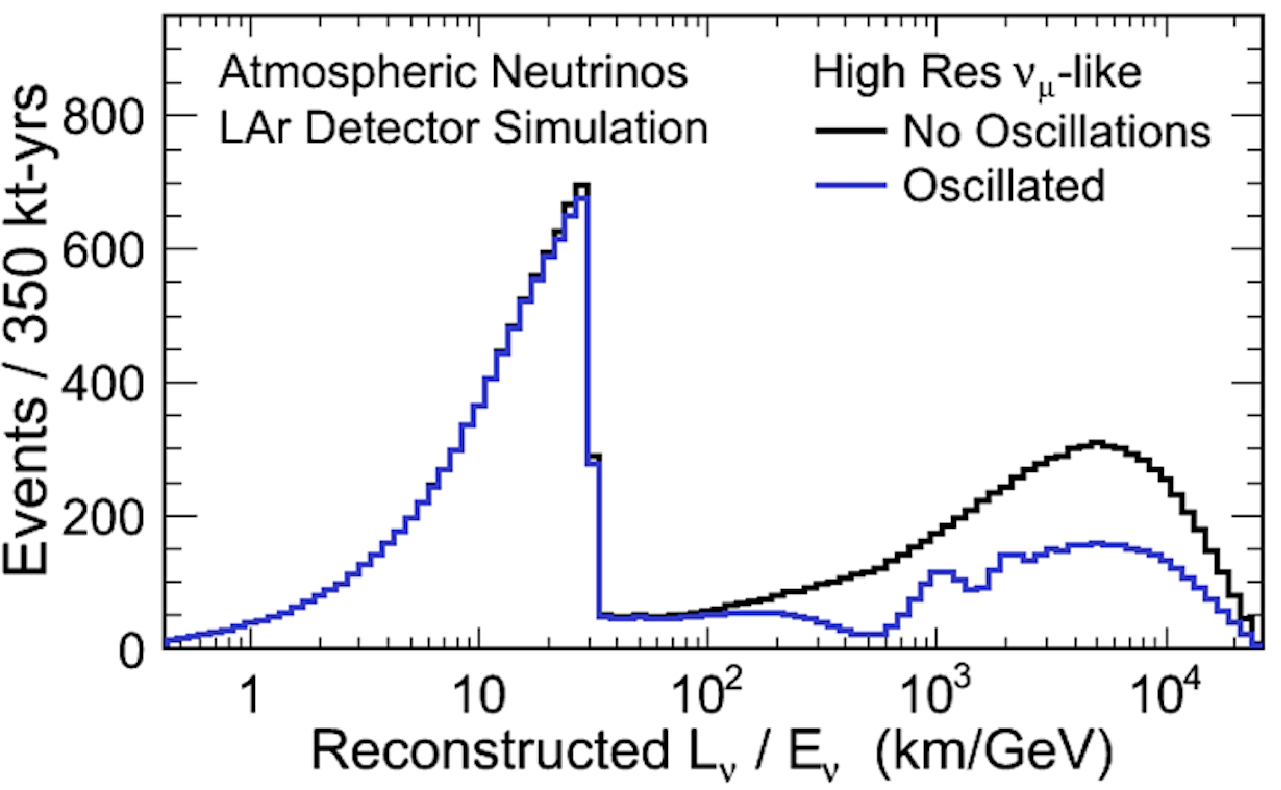
\includegraphics[width=0.4\textwidth]{atm_spectrum_LoverE.pdf}
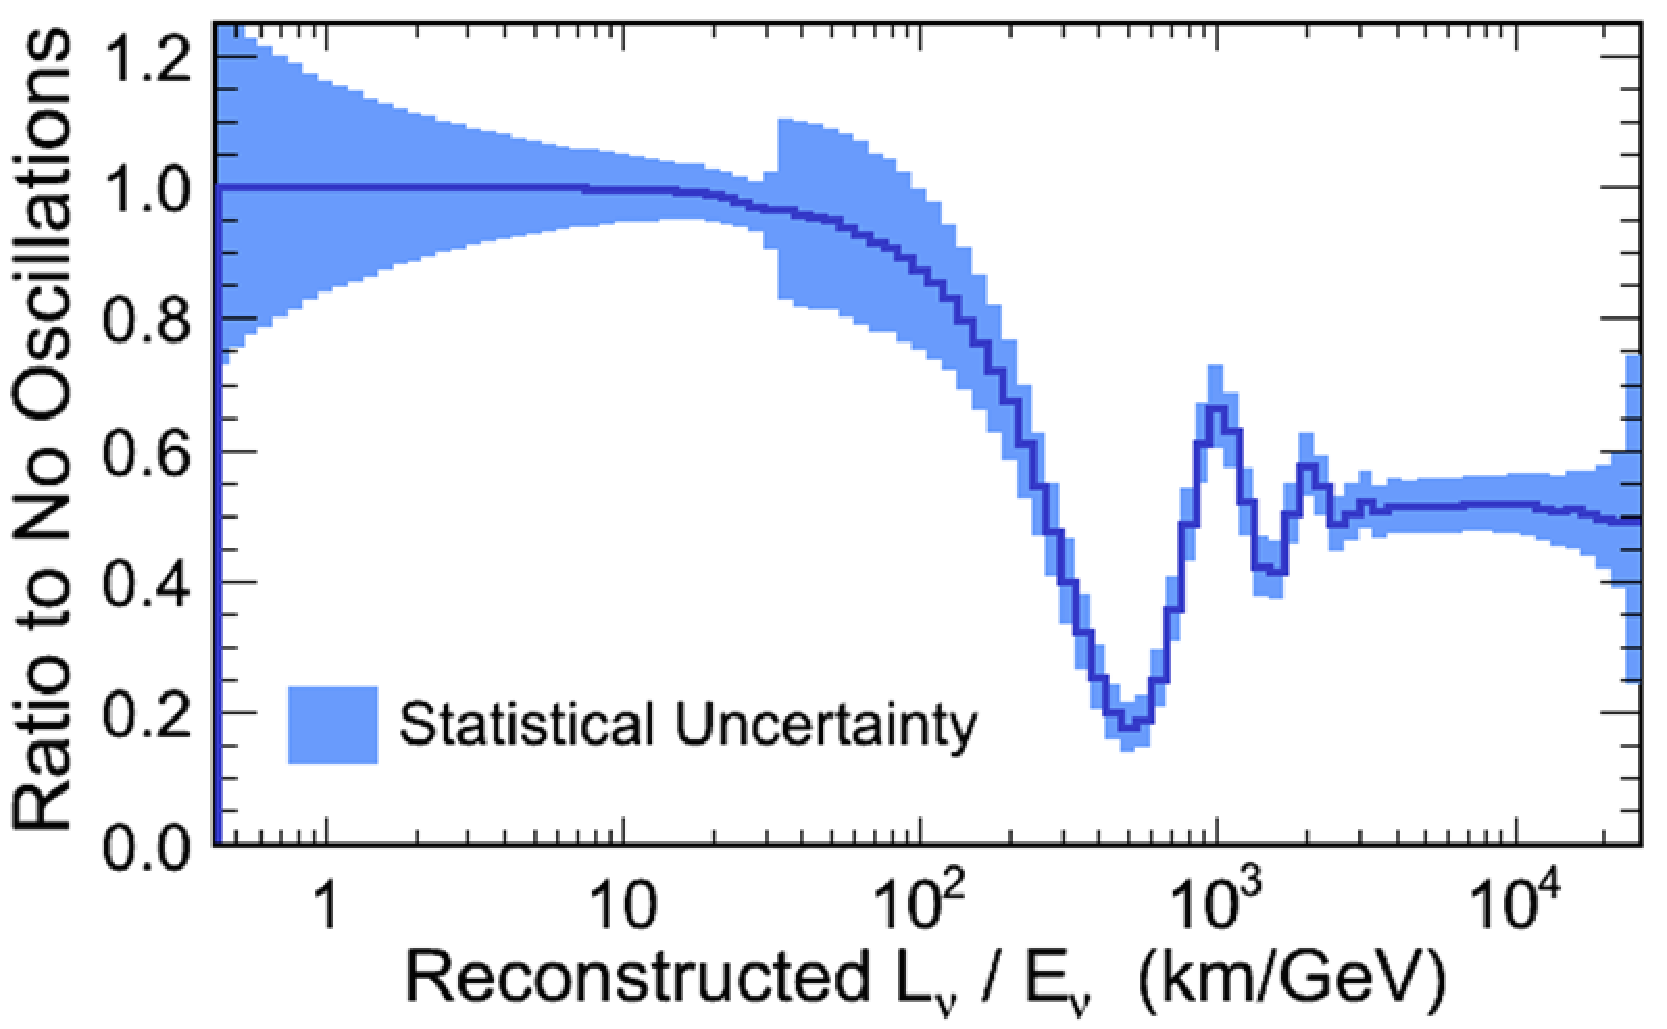
\includegraphics[width=0.4\textwidth]{atm_spectrum_LoverE_2.pdf}
\end{dunefigure}

When neutrinos travel through the Earth, the \dword{msw} resonance influences 
electron neutrinos in the few-GeV energy range. More precisely, the resonance 
occurs for $\nu_e$ in the case of normal mass hierarchy (NH, $\Delta m^2_{32} > 0$) and for 
$\overline{\nu}_e$ in the case of inverted mass hierarchy (IH, $\Delta m^2_{32} < 0$).

The \dword{mh} sensitivity can be greatly enhanced if neutrino and antineutrino events can be 
separated. The DUNE detector will not be magnetized, but its high-resolution 
imaging offers possibilities for tagging features of events that provide statistical 
discrimination between neutrinos and antineutrinos. For the sensitivity calculations, 
%that follow, 
two such tags were included: a proton tag and a decay electron tag. 

Figure~\ref{fig:atm_mh} shows the \dword{mh} sensitivity as a function of the fiducial exposure. 
Over this range of fiducial exposures, the sensitivity essentially follows the square 
root of the exposure, indicating that the measurement is not systematics-limited. 
Unlike beam measurements, the sensitivity to \dword{mh} with atmospheric neutrinos is 
nearly independent of the \dword{cp} violating phase.  The sensitivity comes from both 
electron neutrino appearance as well as muon neutrino disappearance and depends strongly 
 on the true value of $\theta_{23}$, as shown in Figure~\ref{fig:atm_mh}.  Despite the
much smaller mass, \dword{dune} will have sensitivity comparable to \hyperk for atmospheric 
neutrino analyses~\cite{Kearns:2013lea} because of the higher detector resolution.

\begin{dunefigure}
[MH Sensitivity vs. Exposure for Atmospheric Neutrinos]{fig:atm_mh}
{Sensitivity to mass hierarchy using atmospheric neutrinos as a function of fiducial exposure in a liquid argon detector (left) and as a function of the true value of $\theta_{23}$ (right).  For comparison, \hyperk sensitivities are also shown \cite{Kearns:2013lea}.}
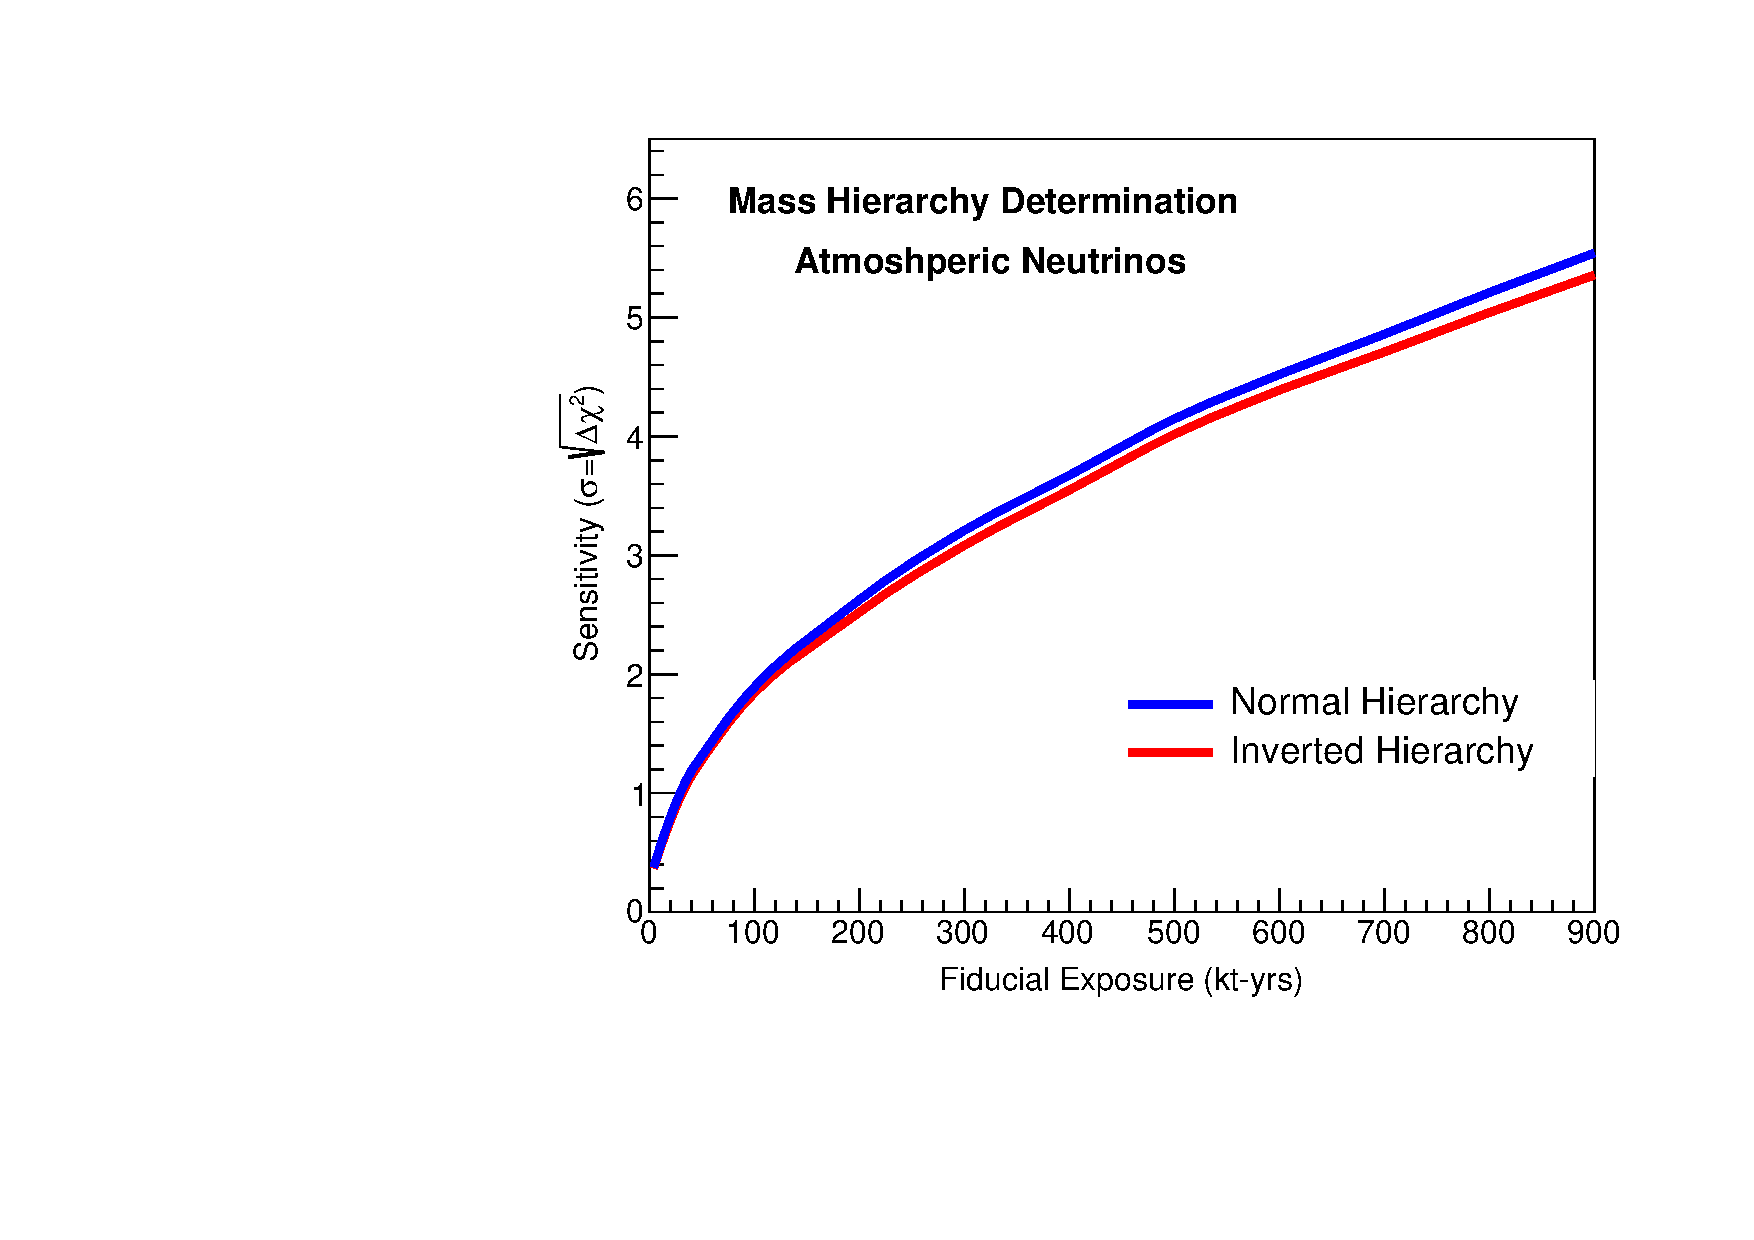
\includegraphics[width=0.42\linewidth]{atm_mh_vs_exposure.pdf}
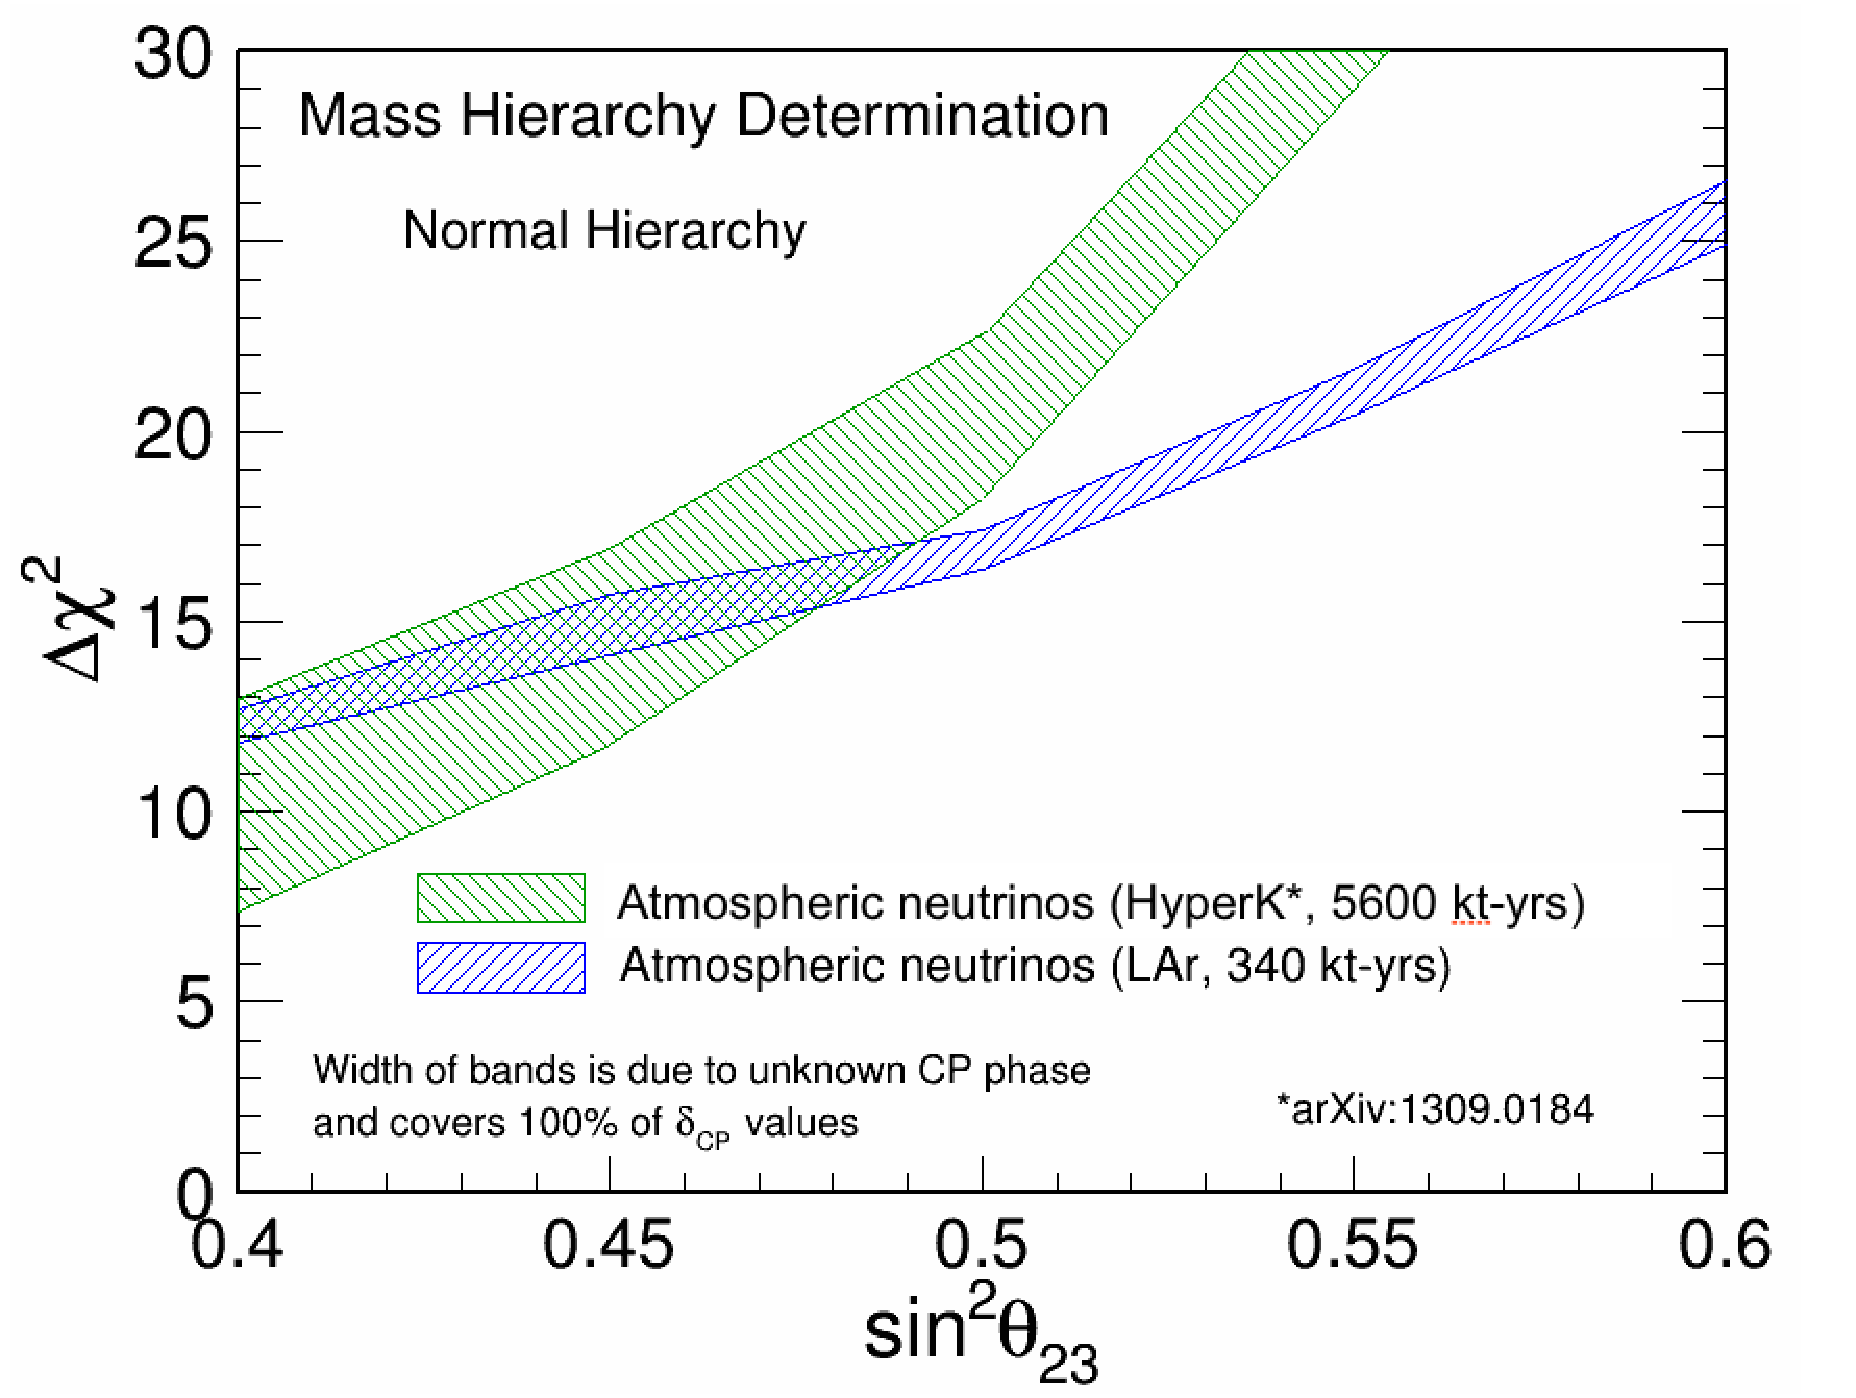
\includegraphics[width=0.48\linewidth]{combined_sensitivity_hierarchy_lbne_vs_hyperk.pdf}
\end{dunefigure}

In the two-flavor approximation, neutrino oscillation probabilities depend on 
$\sin^2(2\theta)$, which is invariant when changing $\theta$ to $\pi/2-\theta$. In this case, the octant 
degeneracy remains for $\theta_{23}$ in the leading order terms of the full 
three-flavor oscillation probability, making it impossible to determine whether $\theta_{23}< \pi/4$ or 
$\theta_{23}> \pi/4$. Accessing full three-flavor oscillation with atmospheric neutrinos 
should help solve the ambiguity.


These analyses will provide an approach complementary to the beam neutrino approach. 
% Atmospheric neutrinos  can help to lift
For instance, atmospheric neutrinos
%\fixme{To what does they refer?}
should resolve 
degeneracies present in beam analyses because % through the fact that 
the \dword{mh} sensitivity is essentially independent of $\delta_{CP}$.   Atmospheric neutrino data will be acquired 
even in the absence of the beam and will provide a useful sample for developing
reconstruction software, analysis methodologies, and calibrations.  
Atmospheric neutrinos provide a window into a range of new physics scenarios, and %can 
may allow \dword{dune} to place limits on Lorentz and \dword{cpt} violation (see Section~\ref{sec:nonaccel-atm-bsm}), 
non-standard interactions~\cite{Chatterjee:2014gxa}, mass-varying neutrinos~\cite{Abe:2008zza}, and
sterile neutrinos~\cite{Abe:2014gda}.

\subsection{BSM Physics with Atmospheric Neutrinos}
\label{sec:nonaccel-atm-bsm}

Studying \dword{dune} atmospheric neutrinos is a promising approach
to searching for Lorentz and \dword{cpt} violation,
which has been hypothesized
to emerge from an underlying Planck-scale theory like strings~\cite{Kostelecky:1988zi,Kostelecky:1991ak}.
The comprehensive realistic effective field theory
for Lorentz and \dword{cpt} violation,
the \dword{sme}~\cite{Kostelecky:1994rn,Colladay:1996iz,Colladay:1998fq,Kostelecky:2003fs},
is a powerful and calculable framework
for analyzing experimental data.
All \dword{sme} coefficients for Lorentz and \dword{cpt} violation
governing the propagation and oscillation of neutrinos
have been enumerated~\cite{Kostelecky:2003cr,Kostelecky:2011gq},
and many experimental measurements of \dword{sme} coefficients 
have been performed to date~\cite{Kostelecky:2008ts}.
Nonetheless,
much of the available \dword{sme} coefficient space 
in the neutrino sector remains unexplored.

Experimental signals predicted by the \dword{sme} include
corrections to standard neutrino-neutrino 
and antineutrino-antineutrino mixing probabilities,
oscillations between neutrinos and antineutrinos,
and modifications of oscillation-free propagation,
all of which incorporate unconventional dependencies
on the magnitudes and directions of momenta and spin.
For \dword{dune} atmospheric neutrinos,
the long available baselines,
the comparatively high energies accessible,
and the broad range of momentum directions
offer advantages that can make possible great
improvements 
in sensitivities to certain types of Lorentz and \dword{cpt} violation~\cite{Kostelecky:2003cr,Kostelecky:2011gq,Kostelecky:2003xn,Kostelecky:2004hg,Diaz:2009qk,Diaz:2013saa,Diaz:2013wia}.
To date,
%three 
experimental searches for Lorentz and \dword{cpt} violation
with atmospheric neutrinos have been published 
by the IceCube and \superk collaborations~\cite{Abbasi:2010kx,Abe:2014wla,Aartsen:2017ibm}.
Similar studies are possible with \dword{dune},
and many \dword{sme} coefficients can be measured that remain unconstrained to date.
%Other prospects of interest include limits from Cherenkov processes
%at long baselines and high energies~\cite{Kostelecky:2011gq}.
%Significant contributions to the search 
%for Lorentz and CPT violation may also 
%come from studies of cosmological neutrinos
%once more is understood about their nature,
%as these offer an extreme baseline
%and correspondingly striking sensitivities
%to SME coefficients~\cite{Diaz:2013wia}.

An example of the potential reach of studies with \dword{dune} atmospheric neutrinos
is shown in Figure \ref{fig:atm},
which displays estimated sensitivities
from \dword{dune} atmospheric neutrinos to a subset of coefficients 
controlling isotropic (rotation-invariant) violations 
in the Sun-centered frame~\cite{Kostelecky:2002hh}.
The experimental sensitivities to these effects
are set primarily by the baseline and the maximum detectable energy.
\dword{dune} can achieve first measurements (red) on some coefficients
and improved measurements (green) on others.
Gray bars show existing limits.

To illustrate an \dword{sme} modification of oscillation probabilities,
consider a measurement of the atmospheric neutrino and antineutrino flux
as a function of energy.
For definiteness,
we adopt atmospheric neutrino fluxes~\cite{Honda:2015fha},
evaluated using the NRLMSISE-00 global atmospheric model~\cite{Picone},
that result from a production event at an altitude of 20 km.
Assuming conventional oscillations with standard mass-matrix values from the
%\fixme{The abbreviation PDG is not in the glossary. I suggest spelling it out unless it is used more than once.}
\dword{pdg}~\cite{Tanabashi:2018oca},
the fluxes at the detector are shown in Figure \ref{fig:atm2}.
The sum of the $\nu_e$ and $\overline\nu_e$ fluxes
is shown as a function of energy as a red dashed line, 
while the sum of the $\nu_\mu$ and $\overline\nu_\mu$ fluxes 
is shown as a blue dashed line. 
Adding an isotropic non-minimal coefficient for Lorentz violation
of magnitude $\mathaccent'27 c^{(6)}_{e \mu} = 10^{-28}$ GeV$^{-2}$
%\fixme{expression with coeff 6 e/mu = ... causes error. Anne  Fixed - Lisa}
changes the fluxes from the dashed lines to the solid ones.
This coefficient is many times smaller
than the current experimental limit.
Nonetheless,
the flux spectrum is predicted to change significantly 
at energies over approximately 100 GeV. 

\begin{dunefigure}[Sensitivity to Lorenz and CPT violation with atmospheric neutrinos]{fig:atm}{Estimated sensitivity to Lorenz and CPT violation with atmospheric neutrinos in the non-minimal isotropic SME. The sensitivities are calculated based on the properties of the atmospheric neutrino flux (baseline and maximum detectable neutrino energy) and have not been analyzed using the DUNE simulation and reconstruction framework.}
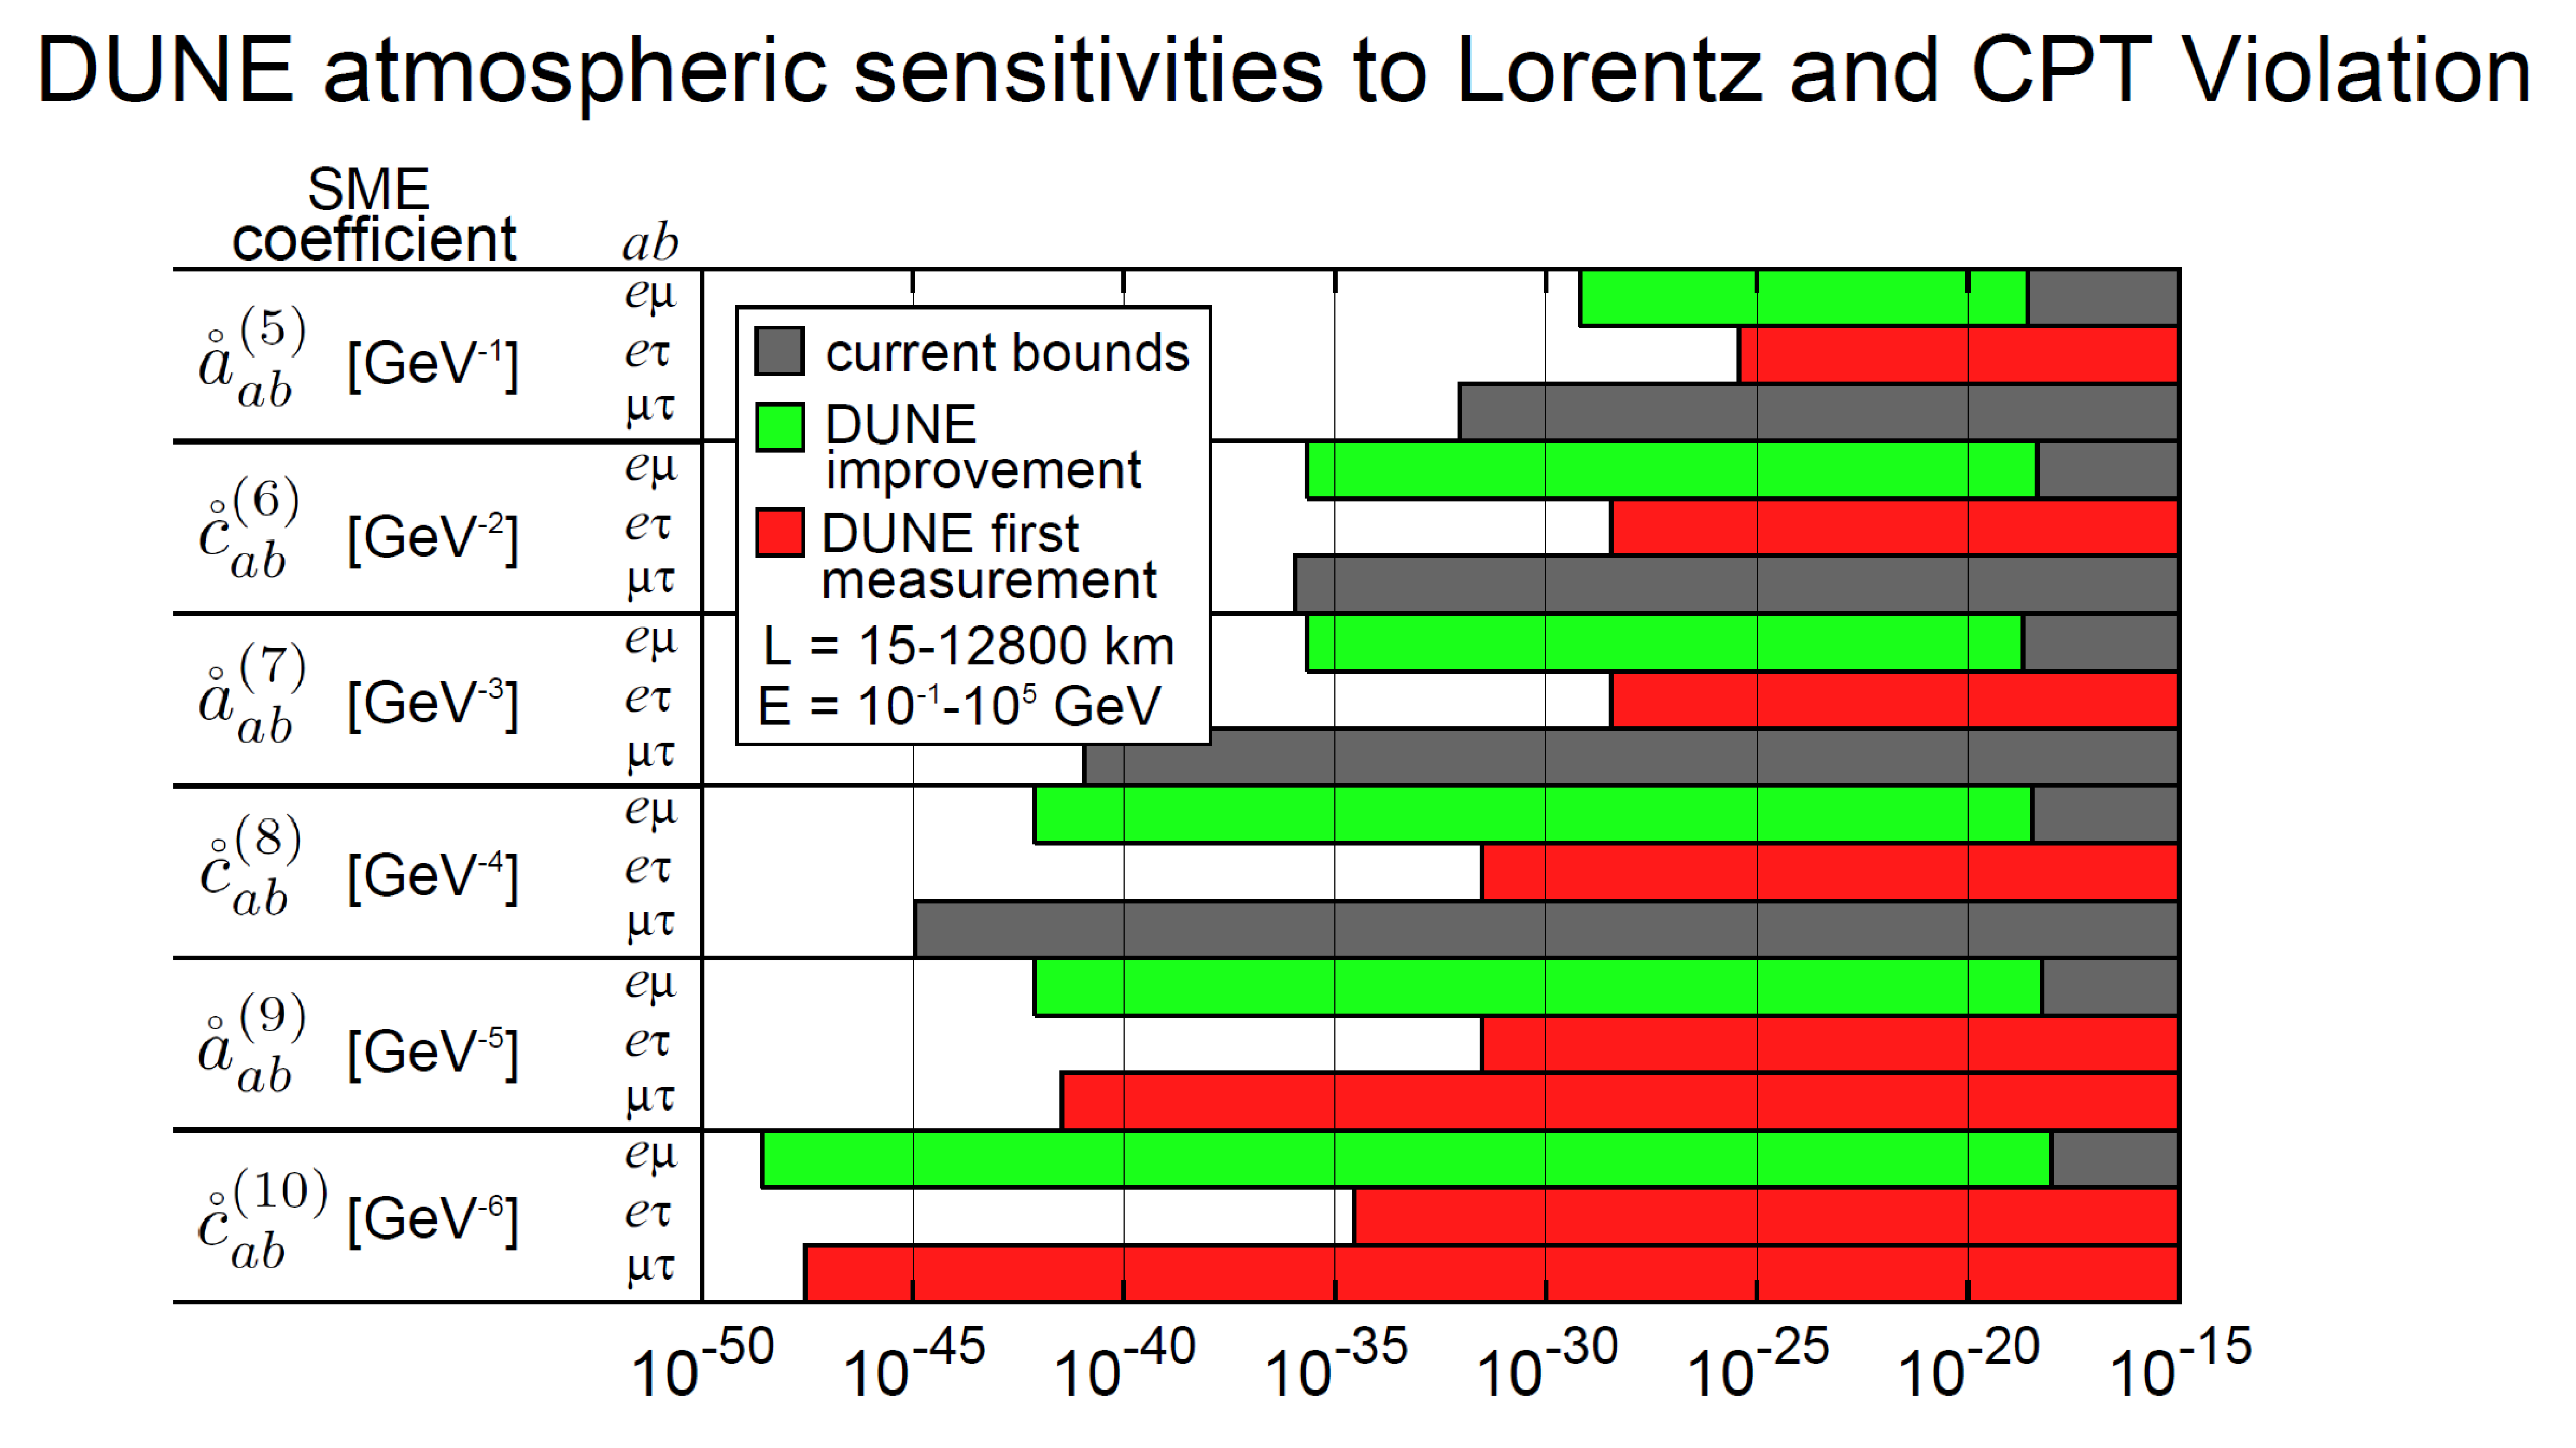
\includegraphics[width=0.8\textwidth]{DUNE-atm.pdf}
\end{dunefigure}

\begin{dunefigure}[Atmospheric fluxes of neutrinos and antineutrinos 
as a function of energy in the non-minimal isotropic SME]{fig:atm2}{Atmospheric fluxes of neutrinos and antineutrinos as a function of energy for conventional oscillations (dashed line) and in the non-minimal isotropic SME (solid line).}
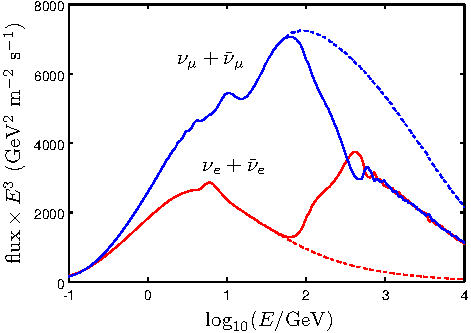
\includegraphics[width=0.8\textwidth]{DUNE-atm2.pdf}
\end{dunefigure}

%\subsection{Reconstruction of atmospheric neutrinos}
%\label{sec:nonaccel-atm-reco}

